\documentclass{article}
\usepackage[paperheight=395pt, paperwidth=240pt, width=166pt, height=294pt, headsep=2pt]{geometry}
\usepackage[noinfo, frame, a5, center, lualatex]{crop}
\usepackage{graphicx}
\usepackage{shandean}
\usepackage{luamplib}
\begin{document}
\pagestyle{empty}
% full title
\centerline{\vbox{\openup 12pt\halign{\hss #\hss\cr
\hbox to 3em{T H E}\cr
\lower 2pt\hbox to 9em{\Large L I F E}\cr
\hbox to 3em{A N D}\cr
\lower 3pt\hbox to 15em{\Large O P I N I O N S}\cr
\textsc{o f}\cr
\hbox{\Large \lsss{TRISTRAM SHANDY},}\cr
\lower-2pt\hbox{\textsc{\lss{Gentleman}.}}\cr
}}}
\vfill
\noindent
\hbox to \textwidth{\footnotesize \textit{Non enim excursus hic ejus, sed opus ipsum est.}\hfill}
\hbox to \textwidth{\footnotesize \hfill \textsc{Plin.} Lib.\@ quintus Epistola sexta.}
\vfill
\centerline{\lsss{VOL}.\quad VII.}
\vfill
\centerline{\lsss{LONDON}:}
\centerline{\small Printed for T.\@ \textsc{Becket} and P.\@ A.\@  \textsc{Dehont},\rlap{\quad\club}}
\centerline{\small in the Strand.\quad M DCC LXV.}

\newpage\null
\vfill
\bgroup\small
\hrule
\bigskip

\centerline{\itshape\lsss{ERRATA}.}

\noindent
Page 33.\@ Vol.\@ VII.\@ last line, dele \textit{and}.\\[2pt]
Page 71.\@ Vol.\@ VII.\@ 3d line instead of striking\\[2pt]
\null\quad read \textit{sticking}\\[2pt]
Page 34.\@ Vol.\@ VIII.\@ 13th line, read \textit{inflam}-\\[2pt]
\null\quad \textit{matory}.

\bigskip
\hrule
\egroup
\vfill
\newpage
\pagestyle{fancy}
\thispagestyle{empty}
\setcounter{page}{1}
\hbox{}\vskip -36pt
\moveright 88pt\vbox to 0pt{\hsize
40pt\rlap{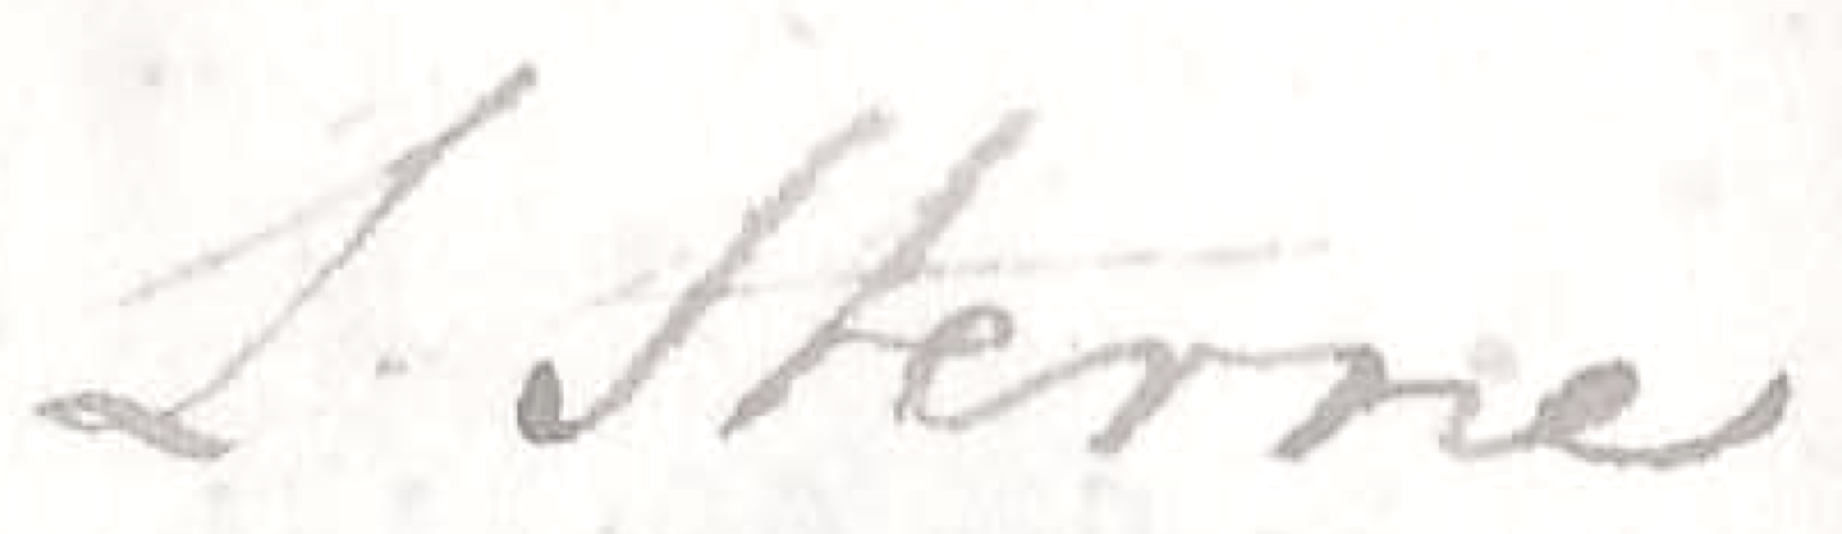
\includegraphics[width=60pt]{sterne.png}}\vss}

\[\vbox{\openup 12pt\halign{\hss # \hss\cr
\addfontfeature{LetterSpace=12.0}\textsc{the}\cr
\large \lsss{LIFE}\enspace and\enspace \lsss{OPINIONS}\cr
\addfontfeature{LetterSpace=12.0}\textsc{of}\cr
\large \ls{TRISTRAM SHANDY}, Gent.\cr}}\]

\vskip 12pt
\hrule

\setlength{\baselineskip}{14pt}  % 21*14 = 294   294/23 \simeq 12.7826 
\sloppy





\section{\lsss{CHAP}.\enspace I.}

\dropcap{N}{o}\tsh I think, I said, I
would write two volumes every year,\break provided the vile cough which
then tormented me, and which to this hour I dread worse than the
devil, would but give me leave\tsk and in another
place\tsk (but where, I can’t recollect now) speaking of my
book as a \textit{machine}, and laying my pen and ruler down
cross-wise\catch{upon} upon the table, in order to gain the greater credit to
it\tsk I swore it should be kept a going at that rate these forty
years, if it pleased but the fountain of life to bless me so long
with health and good spirits.

Now as for my spirits, little have I to lay to their
charge\tsk nay so very little (unless the mounting me upon a long
stick, and playing the fool with me nineteen hours out of the
twenty-four, be accusations) that on the contrary, I have
much\tsk much to thank ’em for:\break 
\stick{cheerily have ye made me tread the path}
of life with all the burdens of it (except its
cares) upon my back; in no one moment of my existence, that I
remember, have ye once deserted me, or tinged the objects which
came in my way, either with\catch{sable,}
\stick{sable, or with a sickly green; in dangers}
\stick{\tight{ye gilded my horizon with hope, and when}}
\textsc{Death} himself knocked at my door\tsk ye bad him
come again; and in so gay a tone of careless indifference, did ye
do it, that he doubted of his commission\tsh

\indent\lqq\tsh There must certainly be some\break\lqq mistake in this
matter,\,” quoth he.

Now there is nothing in this world I abominate worse, than to be
interrupted in a story\tsh and I was that moment telling
Eugenius a most tawdry one in my way, of a nun who fancied
herself a shell-fish, and of a monk damn’d for\break eating a
muscle, and was shewing him the grounds and justice of the
procedure\tsh\patch{\lqq\tsk Did}

\lqq\tsk Did ever so grave a personage\break
\lqq get into so vile a scrape?” quoth\break
Death. Thou hast had a narrow escape,
Tristram, said Eugenius, taking hold of my hand as I
finish’d my story\tsh

But there is no \textit{living}, Eugenius, re-\break plied I, at this
rate; for as this \textit{son of a whore} has found out my
lodgings\tsh

\tsk You call him rightly, said Eugenius,\break
\tsk for by sin, we are told, he enter’d the world\tsh I care not which way he
\stick{enter’d, quoth I, provided he be not in} such a hurry to take me out with him\tsk for
I have forty volumes to write, and forty thousand things to say and do, which no body
in the world will say and do for me, except thyself; and as thou\catch{seest} seest he has got
me by the throat (for\break
Eugenius could scarce hear me speak across the table), and
that I am no match for him in the open field, had I not better, 
whilst these few scatter’d spirits remain, 
\stick{and these two spider legs of mine holding}
\stick{one of them up to him) are able to support} 
me\tsk had I not better, Eugenius, fly for my life? ’tis my
advice, my dear Tristram, said Eugenius\tsk then by heaven! I
will lead him a dance he little thinks of\tsh for I will gallop,
quoth I, without looking once behind me, to the banks of the
\stick{Garonne; and if I hear him clattering} at my heels\tsh
I’ll scamper away to mount Vesuvius\tsh from thence to Jop\-pa,
and from Joppa to the world’s end; where, if he follows me, I
pray God he may break his neck\tsh\patch{\tsh He}

\tsh He runs more risk \textit{there}, said Eugenius,
than thou.

Eugenius’s wit and affection brought blood into the
cheek from whence it had been some months
banish’d\tsh ’twas a vile moment to bid adieu
in; he led me\break to my chaise\tsh \textit{Allons!}\@ said I; the
post boy gave a crack with his whip\tsh off I went like a
cannon, and in half a dozen bounds got into Dover.

\vfill\rightline{\ls{CHAP}.}\eject
\null\kern-\baselineskip
\section{\lsss{CHAP}.\enspace II.}

\dropcap{N}{ow} hang it! quoth I, as I look’d towards the French coast\tsk a man should
know something of his own\break
country too, before he goes abroad\tsh and I never gave a
peep into Rochester church, or took notice of the dock of Chatham, or visited St.\@
Thomas at Canterbury, though they all three laid in\break my way\tsh

\tsk But mine, indeed, is a particular case\tsh

So without arguing the matter further with Thomas o’Becket, or any one else\tsk I
skip’d into the boat, and in five minutes we got under sail and scudded away like
the wind.\patch{Pray,}

Pray, captain, quoth I, as I was going down into the cabin, is a man never overtaken
by \textit{Death} in this passage?

Why, there is not time for a man to be\break
sick in it, replied he\tsh What a cursed\break
lyar! for I am sick as a horse, quoth I,\break already\tsh what a brain!\tsh upside down!\tsh
hey-day! the cells are broke 
\stck{loose one into another, and the blood, and} the lymph,
and the nervous juices, with the fix’d and volatile salts, are all jumbled into one
mass\tsh good \hbox{g\tsk!} every thing turns round in it like a thousand whirl\-pools\tsh I’d
give a shilling to know if\break I shan’t write the clearer for it\tsh

Sick! sick! sick! sick!\tsh\patch{\tsk When}

\tsk When shall we get to land? captain\break
\tsk they have hearts like stones\tsh O~I\break
am deadly sick!\tsh reach me that thing, boy\tsh ’tis the most discomfiting sickness\tsh I wish I
was at the bottom\tsk Madam! how is it with you? Undone! undone! un\tsh O! undone!  sir
\tsh What the first time?\tsh No, ’tis the second, third, sixth, tenth time, sir,\tsh
hey-day\tsk what a trampling over head!\break
\tight{\tsk hollo! cabin boy! what’s the matter\tsk}

The wind chopp’d about! s’Death!\tsk\break
then I shall meet him full in the face.

What luck!\tsk ’tis chopp’d about again, master\tsh O the devil chop it\tsh

Captain, quoth she, for heaven’s sake, let us get ashore.

\vfill\rightline{\ls{CHAP}.}\eject
\null\kern-\baselineskip
\section{\lsss{CHAP}.\enspace III.}

\dropcap{I}{t} is a great inconvenience to a man in a haste, that there are three
distinct roads between Calais and Paris, in behalf of which there
is so much to be said by the several deputies from the towns which lie along them,
that half a day is easily lost in settling which you’ll take.

First, the road by Lisle and Arras, which is the
most about\tsh but most interesting, and instructing.

The second that by Amiens, which you may go, if you
would see Chantilly\tsh

And that by Beauvais, which you may go, if you will.\patch{For}

For this reason a great many chuse to go by Beauvais.

\section{\lsss{CHAP}.\enspace IV.}

\dropcap{\lower-10pt\hbox{\normalsize\large\lqq}N}{ow} before I quit
Calais,\,” a tra-\break vel-writer would say, \lqq it would\break
\lqq not be amiss to give some account of\break
\lqq it.\,”\tsk Now I think it very much amiss\break
\tsk that a man
cannot go quietly through a town and let it alone, when it does not meddle with him,
but that he must be turning about and drawing his pen at every kennel he crosses
over, merely o’ my conscience for the sake of drawing it; because, if we may judge
from what has been wrote of these things, by all who have \textit{wrote and
gallop’d}\tsk or who have \textit{gallop’d and wrote}, which is a different way still;
or who for more expedition\catch{than}
\stick{than the rest, have \textit{wrote-galloping}, which} is
the way I do at present\tsk from the great Addison who did it with his
satchel of school-books hanging at his a\tsk and galling his beast’s crupper at
every stroke\break\tsk there is not a gallopper of us all who might not have gone on ambling
quietly in his own ground (in case he had any), and have wrote all he had to write,
dry\break shod, as well as not.

For my own part, as heaven is my judge, and to which I shall ever make my last
appeal\tsk I know no more of Calais, (except the little my barber told me of it, as he
was whetting his razor) than I do this moment of \textit{Grand Cairo}; for it was
dusky in the evening when I landed, and dark as pitch in the morning when I set out,
and yet by merely know-\catch{ing}
ing what is what, and by drawing this from that in one part of
the town, and by spelling and putting this and that together in another\tsk I would
lay any tra\-velling odds, that I this moment write a chapter upon Calais as
long as my arm; and with so distinct and satisfactory a detail of every item, which
is worth a stranger’s curiosity in the town\tsk that you would take me for the
town clerk of Calais itself\tsk and where, sir, would be the wonder? was not
Democritus, who laughed ten times more than I\tsk town-clerk of
\textit{Abdera?} and was not (I forget his name) who had more discretion than us
both, town-clerk of Ephesus?\tsh it should be penn’d moreover, Sir, with so
much knowledge and good sense, and truth, and precision\tsh\patch{\tsk Nay}

\tsk Nay\tsk if you don’t believe me, you may read the
chapter for your pains.

\section{\lsss{CHAP}.\enspace V.}

\dropcap{C}{alais}, \textit{Calatium, Calusium,\break
Calesium.}

This town, if we may trust it's\sic\ ar\-chives, the authority of which
I see no reason to call in question in this place\tsk was
\textit{once} no more than a small village belonging to one of the
first Counts de Guines; and as it boasts at present of no
less than fourteen thousand inhabitants, exclusive of four hundred
and twenty distinct families in the \textit{basse ville}, or
suburbs\tsh it must have grown up by little and little, I
suppose, to it's\sic\ present size.\patch{Though}

Though there are four convents, there is but one parochial church in the whole town;
I had not an opportunity of taking its exact dimensions, but it is pretty easy to
make a tolerable conjecture of ’em\tsk\break for as there are fourteen thousand
inhabitants in the town, if the church holds them all it must be considerably
large\tsk and if it will not\tsk ’tis a very great pity they have not another\tsk it
is built in form of a cross, and dedicated to the Virgin Mary; the steeple which
has a spire to it, is placed in the middle of the church, and stands upon four
pillars elegant and light enough, but sufficiently strong at the same time\tsk it is
decorated with eleven altars, most of which are rather fine than beautiful. The
great altar is a master-piece in its kind; ’tis of white marble, and as I was
told near sixty feet high\tsk\catch{had} had it been much higher, it had been as high as
mount Calvary itself\tsk therefore, I suppose it must be high enough in all
conscience.

There was nothing struck me more than the great \textit{Square};
tho’ I cannot say\break
\stck{’tis either well paved or well built; but ’tis}\break in the heart of the town, and most of the streets,
especially those in that quarter, all terminate in it; could there
have been a fountain in all Calais, which it seems there
cannot, as such an object would have been a great ornament, it is
not to be doubted, but that the inhabitants would have had it in
the very centre of this square,\tsk not that it is properly a
square,\break\tsk because ’tis forty feet longer from
east to west, than from north to south; so that the French
in general have more\catch{reason} reason on their side in calling them
\textit{Places} than \textit{Squares}, which, strictly speaking, to be
sure they are not.

The town-house seems to be but a sorry building, and not to be
kept in the best repair; otherwise it had been a second great
ornament to this place; it answers however its destination, and
serves very well for the reception of the magistrates, who assemble
in it from time to time; so that ’tis presumable, justice is
regularly distributed.

I have heard much of it, but there is nothing at all curious in
the \textit{Courgain}; ’tis a distinct quarter of the town,
inhabi\-ted solely by sailors and fishermen; it consists of a number
of small streets, neatly built and mostly of brick; ’tis\catch{extremely}
extremely populous, but as that may be accounted for, from the
principles of their diet,\tsk there is nothing curious in that
neither.\tsh A traveller may see it to satisfy
himself\tsk he must not omit however taking notice of \textit{La Tour de Guet}, upon
any account; ’tis so called from its particular destination,
because in war it serves to discover and give notice of the enemies
which approach the place, either by sea or land;\tsh but
’tis monstrous high, and catches the eye so continually, you
cannot avoid taking notice of it, if you would.

It was a singular disappointment to me, that I could not have
permission to take an exact survey of the fortifications, which are
the strongest in the world, and\catch{which,} which, from first to last, that is,
for the time they were set about by Philip of France
Count of Bologne, to the present war, wherein many
reparations were made, have cost (as I learned afterwards from an
engineer in Gascony)\tsk above a hundred millions of
livres. It is very remarkable, that at the \textit{Tête de
Gra\-ve\-lenes}, and where the town is naturally the weakest, they
have expended the most money; so that the outworks stretch a great
way into the campaign, and consequently occupy a large tract of
ground.\break\tsk However, after all that is \textit{said} and
\textit{done}, it must be acknowledged that Calais was never
upon any account so considerable from itself, as from its
situation, and that easy enterance which it gave our ancestors upon
all occasions into France: it was not without its
inconveniences\catch{also;} also; being no less troublesome to the
English in those times, than Dunkirk has been to us,
in ours; so that it was deservedly looked upon as the key to both
kingdoms, which no doubt is the reason that there have arisen so
many contentions who should keep it: of these, the siege of
Calais, or rather the blockade (for it was shut up both by
land and sea) was the most memorable, as it with-stood the efforts
of Edward the third a whole year, and was not terminated at
last but by famine and extream misery; the gallantry of \textit{Eustace
de St.\@ Pierre}, who first offered himself a victim for his
fellow citizens, has rank’d his name with heroes. As it will
not take up above fifty pages, it would be injustice to the reader,
not to give him a\catch{minute} minute account of that romantic transaction, as well
as of the siege itself, in Rapin’s own words:

\section{\lsss{CHAP}.\enspace VI.}

\dropcap{\hbox to 24pt{\Tsk}B}{ut} courage! gentle reader!\break
\tsh I scorn it\tsh ’tis enough\break
to have thee in my power\tsh but to make use of the advantage which the fortune of
the pen has now gained over thee, would be too much\tsh No\tsh !\break
by that all powerful fire which warms the visionary brain, and lights the spirits through
unworldly tracts! ere I would force a helpless creature upon this hard service, and
make thee pay, poor soul! for fifty pages, which I have no right to sell thee,\tsk
naked as\catch{I am,} I am, I would browse upon the mountains, and smile that the north wind
brought me neither my tent or my supper.

\tsh So put on, my brave boy! and make the best of thy way to
Boulogne.

\vfill\rightline{\ls{CHAP}.}\eject
\null\kern-\baselineskip
\section{\lsss{CHAP}.\enspace VII.}

\dropcap[findent=1pt]{\hbox to 24pt{\Tsk}B}{oulogne}!\tsh hah!\break
\tsk so we are all got together\break
\tsh debtors and sinners before heaven;\break
a jolly
set of us\tsk but I can’t stay and quaff it off with
you\tsk I’m pursued myself like a hundred devils, and shall be
overtaken before I can well change horses:\tsh for heaven’s
sake, make haste\tsh ’Tis for high treason, quoth a very little
man, whispering as low as he could to a very tall man that stood next
him\tsh Or else for murder; quoth\break
\stick{the tall man\tsh Well thrown, size-ace!}
quoth I. No; quoth a third, the gen-\break tleman has been
committing\tsh\tsh.\patch{Ah!}

Ah ! ma chere fille ! said I, as she\break
tripp’d by from her matins\tsk you look 
as rosy as the morning (for the sun was
rising, and it made the compliment the 
more gracious)\tsh No; it can’t be that,\break
quoth a fourth\tsh (she made a curt’sy\break
to me\tsk I kiss’d my hand) ’tis debt;
continued he: ’Tis certainly for debt; 
quoth a fifth; I would not pay that 
gentleman’s debts, quoth \textit{Ace}, for a 
thousand pounds; Nor would I, quoth 
\stick{\textit{Size}, for six times the sum\tsk Well thrown,}
Size-Ace, again! quoth I;\tsk but I have\break
no debt but the debt of \textsc{Nature}, and I
want but patience of her, and I will
pay her every farthing I owe her\tsh\break 
How can you be so hard-hearted, \textsc{Ma\-dam}, 
to arrest a poor traveller going 
along without molestation to any one\catch{upon} 
upon his lawful occasions? do stop that
death-looking, long-striding scoundrel of a scare-sinner, who is
posting after\break me\tsh he never would have followed me but
for you\tsh if it be but for a stage, or two, just to give
me start of him, I beseech you, madam\tsh\tsh\break
do, dear lady\tsh.

\tsh Now, in troth, ’tis a great pity, quoth mine
Irish host, that all this good courtship should be lost; for
the young gentlewoman has been after going out of hearing of it all
along\tsh.

\tsh Simpleton! quoth I.

\tsh So you have nothing \textit{else} in Bou\-logne
worth seeing?\patch{\tsk By}

\tsk By Jasus! there is the finest\break
\textsc{Seminary} for the \textsc{Humanities}\tsh.

\tsk There cannot be a finer; quoth I.

\section{\lsss{CHAP}.\enspace VIII.}

\dropcap{W}{hen} the precipitancy of a
man’s wishes hurries on his ideas ninety times faster than
the vehicle he rides in\tsk woe be to truth! and woe be to the
vehicle and its tackling (let ’em be made of what stuff you
will) upon which he breathes forth the disappointment of his
soul!

As I never give general characters either of men or things in
choler, \lqq\textit{the most haste, the worse speed},\,” was
all the re-\catch{flection} flection I made upon the affair, the first time it
happen’d;\tsk the second, third, fourth, and fifth time, I
confined it respectively to those times, and accordingly blamed
only the second, third, fourth, and fifth post-boy for it, without
carrying my reflections further; but the event
continuing to befall me from the fifth, to the sixth, seventh,
eighth, ninth, and tenth time, and without one exception, I then
could not avoid making a national reflection of it, which I do in
these words;

\textit{That something is always wrong in a French post-chaise upon
first setting out}.

Or the proposition may stand thus.

\textit{A French postilion has always to alight\catch{before} before he has got
three hundred yards out of town}.

What’s wrong now?\tsh Diable!\tsh\break
a rope’s broke!\tsh a knot has slipt!\break
\tsh a staple’s drawn!\tsh a bolt’s to whittle!\tsh a tag, a
rag, a jag, a\break strap, a buckle, or a
buckle’s tongue, want altering.\tsh

Now true as all this is, I never think\break myself impower’d to
excommunicate thereupon either the post-chaise, or its
driver\tsh nor do I take it into my head to swear by the
living G\tsk, I would rather go a foot ten thousand
times\tsh or that I will be damn’d if ever I get
into another\tsh but I take the matter coolly
before me, and consider, that some tag, or\catch{rag,} rag, or jag, or bolt, or
buckle, or buckle’s tongue, will ever be a wanting, or want
altering, travel where I will\tsk so\break I never chaff, but take the
good and the bad as they fall in my road, and get
on:\tsh Do so, my lad! said I; he had lost five minutes
already, in alighting in order to get at a luncheon of black bread,
which he had cramm’d\break into the chaise-pocket, and was
remounted and going leisurely on, to relish it the
better.\tsh Get on, my lad, said I, briskly\tsk but in
the most persuasive tone imaginable, for I jingled a
four and twenty sous piece against the glass, taking care to hold
the flat side towards him, as he look’d back: the dog
grinn’d intelligence from his right ear to his left, and
behind his sooty\catch{muzzle} muzzle discover’d such a pearly row of teeth, that
\textit{Sovereignty} would have pawn’d her jewels for
them.\tsh

\noindent
Just heaven! $\Big\{\vcenter{\halign{#\hss\cr What masticators!\tsh\cr What bread!\tsh\cr}}$

\noindent
and so, as he finish’d the last mouthful of it, we
enter’d the town of Montreuil.

\vfill\rightline{\ls{CHAP}.}\eject
\null\kern-\baselineskip
\section{\lsss{CHAP}.\enspace IX.}

\dropcap{T}{here} is not a town in all France, which in my opinion, looks better in the
map, than \textsc{Montreuil};\tsh I own, it does not look so well in the book of
post roads; but when you come to see it\tsk to be sure it looks most pitifully.

There is one thing however in it at present very handsome; and that is the
inn-keeper’s daughter: She has been eighteen months at Amiens, and six at
Paris, in going through her classes; so knits, and sews, and dances, and
does the little coquetries very well.\tsh

\tsk A slut! in running them over with\-in these five minutes
that I have stood looking at her, she has let fall at least a\catch{dozen} dozen
loops in a white thread stocking\break
\tsh Yes, yes\tsk I see, you cunning gipsy!\break
\tsk ’tis long, and taper\tsk you need
not pin it to your knee\tsk and that ’tis your
own\tsk and fits you exactly.\tsh

\tsk That Nature should have told this creature a word
about a \textit{statue’s thumb!}\tsh

\tsk But as this sample is worth all their thumbs\tsh besides I
have her thumbs and fingers in at the bargain if they can be
any guide to me,\tsk and as \textit{Janatone} withal (for that
is her name) stands so well for a drawing\tsh may\break I never draw
more, or rather may I draw like a draught-horse, by main
strength all the days of my life,\tsk if I do not draw her in
all her proportions, and\catch{with} with as determin’d a
pencil, as if I had her in the wettest drapery.\tsh

\noindent
\stick{\indent\tight{\tsk But your worships chuse rather that I}}\break give you the length, breadth, and
per-\break
pendicular height of the great parish church, or drawing of the fascade of the
abbey of Saint Austreberte which has been transported from Artois
hither\tsk every thing is just I suppose as the masons and carpenters left them,\tsk and
if the\break
belief in Christ continues so long, will be\break
so these fifty years to come\tsk so your\break
\stck{worships and reverences, may all measure}\break
them at your leisures\tsk but he who\break
measures thee, Janatone, must do it now\break
\tsk thou carriest the
principles of change within thy frame; and considering the chances of a transitory
life, I would not\break answer for thee a moment; and\sic\ e’er\catch{twice}
\stick{twice twelve months are pass’d and gone,}
\stick{thou mayest grow out like a pumkin,}
\stick{and lose thy shapes\tsk or, thou mayest}
go off like a flower, and lose thy beauty\break
\tsk nay, thou mayest go off like a hussy\break
\tsk and lose thyself.\tsk I would not answer for my aunt Dinah, was she alive\tsh
’faith, scarce for her picture\tsh were it but painted by Reynolds\tsk

\tsk But if I go on with my drawing, after naming that son of
Apollo, I’ll be shot\tsh

So you must e’en be content with the original; which, if the evening is fine in
passing thro’ Montreuil, you will see at your chaise door, as you change horses: but
unless you have as bad a reason for haste as I have\tsk you had better stop:\tsk\catch{\tsk She}
\tsk She has a little of the \textit{devote:} but\break
that, sir, is a terce to a nine in your\break
favour\tsh

\tsk\ L\tsk\ help me! I could not count a single point: so
had been piqued, and repiqued, and capotted to the devil.

\section{\lsss{CHAP}.\enspace X.}

\dropcap{A}{ll} which being considered, and\break
that Death moreover might be\break
much nearer me than I imagined\tsh\break
I wish I was at Abbeville, quoth I,
were it only to see how they card and spin\tsh so off we
set.

\noindent
\stick{\lower-3pt\hbox{\ast}\ \textit{de Montreuil a Nampont} \crfill \hbox to 50pt{\textit{poste et demi}\hfill}}\break
\stick{\textit{de Nampont} a Bernay          \crfill \hbox to 50pt{poste\hfill}}

\bgroup\footnotesize
\noindent\quad\lower-2pt\hbox{\ast}\ Vid.\@ Book of French post-roads, page 36.\break
edition of 1762.
\par\egroup
\rightline{de}
\eject
\noindent
\stick{de Bernay a Nouvion             \crfill \hbox to 50pt{poste\hfill}}
\stick{de Nouvion a \textsc{Abbeville} \crfill \hbox to 50pt{poste\hfill}}

\noindent
\tsh but the carders and spinners were all gone to bed.

\bigskip

\section{\lsss{CHAP}.\enspace XI.}

\dropcap{W}{hat} a vast advantage is travelling!
only it heats one; but there is a remedy for that, which you may
pick out of the next chapter.

\vfill\rightline{\ls{CHAP}.}\eject
\null\kern-\baselineskip
\section{\lsss{CHAP}.\enspace XII.}

\dropcap{W}{as} I in a condition to stipulate with
death, as I am this moment with my apothecary, how and where I
will take his glister\tsh I should certainly declare against
submitting to it before my friends; and therefore, I never
seriously think upon the mode and manner of this great
catastrophe, which generally takes up and torments my thoughts
as much as the catastrophe itself, but I constantly draw the
curtain across it with this wish, that the Disposer of all
things may so order it, that it happen not to me in my own
house\tsh but rather in some decent inn\tsh at home, I know
it,\tsh the concern of my friends, and the last services of
wiping my brows and smoothing my\catch{pillow,} pillow, which the quivering
hand of pale affection shall pay me, will so crucify my soul,
that I shall die of a distemper which my physician is not aware
of: but in an inn, the few cold offices I wanted, would be
purchased with a few guineas, and paid me with an undisturbed,
but punctual attention\tsh but mark.  This inn, should not be
the inn at Abbeville\break\tsh if there was not another inn in
the universe, I would strike that inn out of the capitulation:
so

Let the horses be in the chaise exactly by four in the
morning\tsh Yes, by four, Sir,\tsh or by
Genevieve! I’ll raise a clatter in the house, shall
wake the dead.

\vfill\rightline{\ls{CHAP}.}\eject
\null\kern-\baselineskip
\section{\lsss{CHAP}.\enspace XIII.}

\dropcap{\lower-10pt\hbox{\large“}\textit{M}}{\textit{ake}} 
\textit{them like unto a wheel},\,”\break
is a bitter sarcasm, as all the\break
learned know, against the \textit{grand tour}, 
and that restless spirit for making it,\break
\stck{which David prophetically foresaw would}\break haunt the
children of men in the latter days; and therefore, as thinketh the great bishop
Hall, ’tis one of the se\-ver\-est imprecations which
David ever utter’d against the enemies of the
Lord\tsk and, as if he had said, \lqq I wish them no\break
\lqq worse luck than always to be rolling\break
\lqq about\,”\tsk So much
motion, continues he, (for he was very corpulent)\tsk is so much
unquietness; and so much of\catch{rest,} rest, by the same analogy, is so much
of heaven.

Now, I (being very thin) think differently; and that so much of
motion, is so much of life, and so much of joy\break
\tsh and
that to stand still, or get on but slowly, is death and the
devil\tsh

Hollo! Ho!\tsh the whole world’s
asleep!\tsh bring out the horses\tsh grease the
wheels\tsh tie on the mail\tsh and drive a nail
into that moulding\tsh I’ll not lose a
moment\tsh

Now the wheel we are talking of, and \textit{whereinto} (but not
\textit{whereonto}, for that would make an Ixion’s wheel of it)
he curseth his enemies, according to the\catch{bishop’s}
bishop’s habit of body, should certainly be a post-chaise wheel, whether they were
set up in Palestine at that time or not\tsh and my wheel, for the contrary reasons,
must as certainly be a cart-wheel groaning round its revolution once in an age; and
of which sort, were I to turn commentator, I should make no scruple to affirm, they
had great store in that hilly country.

I love the Pythagoreans (much more than ever I dare tell my dear Jenny) for\break
\stick{their \lqq\small χωρισμὸν ἀπὸ τοῦ Σώματος, εἰς’ τὸ}\break
\lqq {\small Καλῶς Φιλοσοφεῖν}\,”\tsh [their] \lqq \textit{getting}\break
\lqq \textit{out of the body, in order to think}\break
\lqq \textit{well}.\,” No man thinks right whilst he is in it; blinded as
he must be, with his congenial humours, and drawn dif-\catch{ferently} ferently aside, as the bishop
and myself have been, with too lax or too tense a fibre\tsh \textsc{Reason} is,
half of it, \textsc{Sense}; and the measure of heaven itself is but the measure of
our present appetites and concoctions.\tsh

\tsh But which of the two, in the present case, do you
think to be mostly in the wrong?

You, certainly\thinspace: quoth she, to disturb a whole family so
early.

\vfill\rightline{\ls{CHAP}.}\eject
\null\kern-\baselineskip
\section{\lsss{CHAP}.\enspace XIV.}

\quad\tsh But she did not know I was un-\break
der a vow not to shave my beard till I\break
got to Paris;\tsh yet I hate to make\break
mysteries of nothing;\tsh ’tis the cold\break
cautiousness of one of those little souls\break
from which \textit{Lessius} (\textit{lib.\@ 13.\@ de moribus\break
divinis, cap.\@ 24.}) hath made his esti-\break
mate, wherein he setteth forth, That\break
one Dutch mile, cubically multiplied,\break
will allow room enough, and to spare,\break
for eight hundred thousand millions,\break
which he supposes to be as great a num-\break
ber of souls (counting from the fall of\break
Adam) as can possibly be damn’d to\break
the end of the world.\patch{From}

From what he has made this second estimate\tsh unless
from the parental goodness of God\tsk I don’t know\tsk I
am much more at a loss what could be in Franciscus
Ribbera’s head, who pretends that no less a space than
one of two hundred Italian miles multiplied into itself,
will be sufficient to hold the like number\tsh he
certainly must have gone upon some of the old Roman souls,
of which he had read, without reflecting how much, by a gradual and
most tabid decline, in the course of eighteen hundred years, they
must unavoidably have shrunk, so as to have come, when he wrote,
almost to nothing.\patch{In}

In Lessius’s time, who seems the cooler man, they
were as little as can be imagined\tsh

\tsh We find them less \textit{now}\tsh

And next winter we shall find them less again; so that if we go
on from little to less, and from less to nothing, I\break hesitate not
one moment to affirm, that in half a century, at this rate, we shall
have no souls at all; which being the period beyond which I doubt
likewise of the existence of the Christian faith, ’twill be
one advantage that both of ’em will be exactly worn out
together.\tsh

Blessed Jupiter! and blessed every other heathen god and goddess! for\catch{now} now ye will
all come into play again, and with Priapus at your tails\tsh\break what jovial times!\tsh
but where am I? and into what a delicious riot of things am I rushing? I\tsh I
who\break
must be cut short in the midst of my days, and taste no more of ’em than what I
borrow from my imagination\tsh peace to thee, generous fool!\break and let me go on.

\vfill\rightline{\ls{CHAP}.}\eject
\null\kern-\baselineskip
\section{\lsss{CHAP}.\enspace XV.}

\quad\tsh \lqq So hating, I say, to make\break
mysteries
of \textit{nothing}\,”\tsh I intrusted it with the
post-boy, as soon as ever I got off the stones; he gave a crack
with his whip to balance the compliment;\break
and with the thill-horse
trotting, and a sort of an up and a down of the other,\break
we danced it along to \textit{Ailly au clochers}, famed in days
of yore for the finest chimes in the world; but we danced
through it without music\tsk the chimes being greatly out of
order\tsk (as in truth they were through all France).

And so making all possible speed, from

\noindent
\textit{Ailly au clochers}, I got to Hixcourt,\\
\rightline{from}
\newpage\noindent
from Hixcourt I got to Pequignay, and\\
from Pequignay, I got to \textsc{Amiens},\\[4pt]
concerning which town I have nothing to inform you, but what I have
informed you once before\tsh and that was\tsh that
Janatone went there to school.

\section{\lsss{CHAP}.\enspace XVI.}

\dropcap{I}{n} the whole catalogue of those
whiff\-ling vexations which come puffing across a man’s
canvass, there is not one of a more teasing and tormenting nature,
than this particular one which I am going to
describe\tsh and for which (unless you travel with an
avance-courier, which numbers do in order to prevent
it)\tsh there is no help: and it is this.

That be you in never so kindly a pro-\break
pensity to sleep\tsh tho’ you are passing\catch{perhaps} perhaps through the
finest country\tsk upon the best roads,\tsk and in the easiest
carriage for doing it in the world\tsh nay, was you sure you could sleep fifty miles straight
forwards, without once opening your eyes\tsk nay what is more,
was you as demonstratively satisfied as you can be of any truth in
Euclid, that you should upon all accounts be full as well
asleep as awake\tsh nay perhaps better\tsh\break
Yet the incessant returns of paying for the horses at every
stage,\tsh with the necessity thereupon of putting your
hand into your pocket, and counting out from thence, three livres
fifteen sous (sous by sous) puts an end to so much of the project,
that you cannot execute above six miles of it (or supposing it is a
post and a half, that is but nine)\tsh were it to save
your soul from destruction.\patch{\tsh I’ll}

\tsh I’ll be even with ’em, quoth I,\break
for I’ll put the precise sum into a piece\break
of paper, and hold it ready in my hand\break
all the way: \lqq Now I shall have no-\break
\lqq thing to do,\,” said I (composing my-\break
self to rest), \lqq but to drop this gently\break
\lqq into the post-boy’s hat, and not say\break
\lqq a word.\,”\tsh Then there wants two\break
sous more to drink\tsh or there is a
twelve sous piece of Louis XIV.\@ which will not pass\tsk or a livre and some odd liards
to be brought over from the last stage, which Monsieur had forgot; which
altercations (as a man cannot dispute very well asleep) rouse him: still is sweet
sleep retrievable; and still might the flesh weigh down the spirit, and recover
itself of these blows\tsk but then, by heaven!\catch{you}
you have paid but for a single post\break
\tsk whereas ’tis a post and a half; and this obliges you to pull out your book of
post-roads, the print of which is so very small, it forces you to open your eyes,
whether you will or no: then Monsieur le Curè offers you a pinch of snuff\tsh\break
or a poor soldier shews you his leg\tsh\break
or a shaveling his box\tsh or the priest-\break
esse of the
cistern will water your wheels\break\tsh they do not want it\tsh but she\break
swears by her \textit{priesthood} (throwing it back) that they do:\tsh then you have all these
points to argue, or consider over in your mind; in doing of which, the rational
powers get so thoroughly awakened\tsh you may get ’em to sleep again as you can.\patch{It}

It was entirely owing to one of these misfortunes, or I had
pass’d clean by the stables of
Chantilly\tsh

\tsh But the postillion first affirming, and then
persisting in it to my face, that there was no mark upon the two
sous piece, I open’d my eyes to be convinced\break
\tsk and seeing
the mark upon it as plain as my nose\tsk I leap’d out of
the chaise in a passion, and so saw every thing at Chantilly
in spite.\tsh I tried it but for three posts and a half,
but believe ’tis the best principle in the world to travel
speedily upon; for as few objects look very inviting in that
mood\tsk you have little or nothing to stop you; by which means
it was that I pass’d through St.\catch{Dennis,} Dennis, without turning my
head so much as on one side towards the Abby\tsh

\tsh Richness of their treasury! stuff and nonsense!\tsh bating their jewels, which are
all false, I would not give three sous for any one thing in it, but \textit{Jaidas’s
lantern}\tsh nor for that either,\break only as it grows dark, it might be\break of use.

\vfill\rightline{\ls{CHAP}.}\eject
\null\kern-\baselineskip
\section{\lsss{CHAP}.\enspace XVII.}

\dropcap{C}{rack}, crack\tsh crack, crack\break\tsh crack, crack\tsk so this is Paris!  quoth I
(continuing in the same mood)\tsk and this is Paris!\tsh humph!\break
\tsh Paris! cried I, repeating the name the third time\tsh

The first, the finest, the most brilliant\tsh

\tsk The streets however are nasty;

But it looks, I suppose, better than it smells\tsh crack, crack\tsh crack, crack\tsh
What a fuss thou makest!\tsk\break
as if it concern’d the good people to be inform’d, That a
man with pale face,\catch{and} and clad in black, had the honour to be driven into Paris at nine
o’clock at night, by a postillion in a tawny yellow jerkin, turned up with red
calamanco\tsk crack, crack\tsh crack, crack\tsh crack, crack,\break
\tsh I wish thy whip\tsh

\tsh But ’tis the spirit of thy nation; so crack\tsk crack on.

Ha!\tsh and no one gives the wall!\break
\tsh but in the \textsc{School} of \textsc{Urbanity}\break
herself, if the walls are besh—t\tsk how can you do otherwise?

And prithee when do they light the lamps? What?\tsk never in the summer months!\tsh
Ho!  ’tis the time of sallads.\break\tsh O rare! sallad and soup\tsk soup and sallad\tsk
sallad and soup, \textit{encore}\tsh\patch{\tsh ’Tis}

\tsh ’Tis \textit{too much} for sinners.

Now I cannot bear the barbarity of it;\break
how can that unconscionable coachman talk so much bawdy to that lean horse?\break
don’t you see, friend, the streets are so villanously narrow, that there is not room in
all Paris to turn a wheel-barrow?\break
In the grandest city of the whole world, it would
not have been amiss, if they had been left a thought wider; nay were it only so
much in every single street, as that a man might know (was it only for satisfaction)
on which side of it he was walking.

\noindent
\stick{\indent One—two—three—four—five—six\tsk}\break
seven\tsk eight\tsk nine\tsk ten.\tsk Ten cook’s
shops! and twice the number of barbers! and all within three minutes driving!\catch{one}
\stick{one would think that all the cooks in the}
\stick{world on some great merry-meeting with}
\stick{the barbers, by joint consent had said\tsk}
\stick{Come, let us all go live at Paris: the}
\stick{French love good eating\tsh they are all}
\stick{\textit{gourmands}\tsh we shall rank high; if}
\stick{their god is their belly\tsh their cooks}
\stick{must be gentlemen: and forasmuch as}
\stick{\textit{the periwig maketh the man}, and the peri-}
\stick{wig-maker maketh the periwig\tsk ergo,}
\stick{would the barbers say, we shall rank}
\stick{higher still\tsk we shall be above you all\tsk}
\stick{we shall be \fnast\  Capitouls at least\tsk pardi!}
we shall all wear swords\tsh

\tsk And so, one would swear, (that is by candle-light,\tsk but there is no depending
upon it) they continued to do, to this day.

\bgroup\footnotesize\indent\fnast\enspace
Chief Magistrate in Toulouse, \&c. \&c. \&c.\par\egroup

\vfill\rightline{\ls{CHAP}.}\eject
\null\kern-\baselineskip
\section{\lsss{CHAP}.\enspace XVIII.}

\dropcap{T}{he} French are certainly misunderstood:\tsh but whether the fault is theirs,
in not sufficiently explaining themselves; or speaking with that exact limitation
and precision which one would expect on a point of such importance, and which
moreover, is so likely to be contested by us\tsh or whether the fault may not be
altogether on our side, in not understanding their language always so critically as
to know “what they would be at”\tsh I shall not decide; but ’tis evident to me, when
they affirm, “\textit{That they who have seen Paris, have seen every thing},” they
must mean to speak of those who have seen it by day-light.\patch{As}

As for candle-light\tsk I give it up\tsh{} I~have said
before, there was no depending upon it\tsk and I repeat it again;
but not because the lights and shades are too sharp\tsk or the
tints confounded\tsk or that there is neither beauty or keeping,
\&c.\break
\stick{. . . for that’s not truth\tsk but it is an un-}
certain light in this respect, That in all the five
hundred grand Hôtels, which they number up to you in
Paris\tsk and the five hundred good things, at a modest
computation (for ’tis only allowing one good thing to a
Hôtel), which by candle-light are best to be \textit{seen, felt,
heard, and understood} (which, by the bye, is a quotation
from Lilly)\tsh the devil a one of us out of fifty,
can get our heads fairly thrust in amongst them.\patch{This}

This is no part of the French computation: ’tis
simply this.

That by the last survey taken in the year one thousand seven
hundred and sixteen, since which time there have been considerable
augmentations, Paris doth contain nine hundred streets;
(viz.)\\[2pt]
In the quarter called the \textit{City}\tsk there are\bnq fifty three streets.\\
In St.\@ \textit{James} of the Shambles, fifty five\bnq streets.\\
In St.\@ \textit{Oportune}, thirty four streets.\\
In the quarter of the \textit{Louvre}, twenty five\bnq streets.\\
In the \textit{Palace Royal}, or St.\@ \textit{Honorius},\bnq forty nine streets.\\
In \textit{Mont.\@ Martyr}, forty one streets.\\
In St.\@ \textit{Eustace}, twenty nine streets.\\
\rightline{In}
\newpage\noindent
In the \textit{Halles}, twenty seven streets.\\
In St.\@ \textit{Dennis}, fifty five streets.\\
In St.\@ \textit{Martin}, fifty four streets.\\
In St.\@ \textit{Paul}, or the \textit{Mortellerie}, twenty\bnq seven streets.\\
The \textit{Greve}, thirty eight streets.\\
In St.\@ \textit{Avoy}, or the \textit{Verrerie}, nineteen\bnq streets.\\
In the \textit{Marais}, or the \textit{Temple}, fifty two\bnq streets.\\
In St.\@ \textit{Antony}’s, sixty eight streets.\\
In the \textit{Place Maubert}, eighty one streets.\\
In St.\@ \textit{Bennet}, sixty streets.\\
In St.\@ \textit{Andrews de Arcs}, fifty one streets.\\
In the quarter of the \textit{Luxembourg}, sixty\bnq two streets.\\[2pt]
And in that of St.\@ Germain, fifty five streets, into any of
which you may walk; and that when you have seen them with\catch{all} all that
belongs to them, fairly by daylight\tsk their gates, their
bridges, their \stick{squares, their statues - - - - and have cru-}\break
\stick{\tight{saded it moreover, through all their parish}}\break
churches, by no means omitting
St.\@ \textit{Roche}\break
\stick{and \textit{Sulpice} - - - and to crown all, have}
taken a walk to the four palaces, which you may see, either with or
without the statues and pictures, just as you chuse\tsk

\tsh Then you will have seen\tsh

\tsh but, ’tis what no one needeth to tell you,
for you will read of it yourself upon the portico of the
Louvre, in these words,\\[3pt]
\lower-3pt\hbox{\ast} \textsc{Earth no such folks!\tsk no folks\bnq\quad e’er such a
town}\\
\textsc{As Paris is!\tsk sing, derry, derry,\bnq\quad down}.

\bgroup\footnotesize
\noindent\lower-3pt\hbox{\ast} Non Orbis gentem, non urbem gens habet
ullam\bnq\qquad\tsh\tsh\tsh\tsh ulla parem.
\par\egroup
\etp\rightline{The}
\newpage
\noindent
The French have a \textit{gay} way of treating every thing
that is Great; and that is all can be said upon it.



\section{\lsss{CHAP}.\enspace XIX.}

\dropcap{I}{n} mentioning the word \textit{gay} (as in\break
the close of the last chapter) it puts one (\textit{i}.\@ \textit{e}.\@ an
author) in mind of the word \textit{spleen}\tsh especially
if he has any thing to say upon it: not that by any
analysis\break\tsk or that from any table of interest or\break genealogy,
there appears much more ground of alliance betwixt them, than
\stick{betwixt light and darkness, or any two} 
\stick{of the most unfriendly opposites in na-}
\stick{ture\tsh only ’tis an undercraft of au-}
\stick{thors to keep up a good understanding}
\stck{amongst words, as politicians do amongst}\break
men\tsk not knowing how near they may\catch{be} be
under a necessity of placing them to each other\tsh which
point being now gain’d, and that I may place mine exactly to
my mind, I write it down here\tsh

\bigskip
\centerline{\lsss{SPLEEN}.}

This, upon leaving Chantilly, I declared to be the best principle in the world to
travel speedily upon; but I gave it only as matter of opinion. I still continue in
the same sentiments\tsk\break only I had not then experience enough of its working to add
this, that though you do get on at a tearing rate, yet you get on but uneasily to
yourself at the same time; for which reason I here quit it entirely, and for ever,
and ’tis heartily at any one’s service\tsk it has spoiled me the digestion of a good
supper, and brought\catch{on} on a bilious diarrhæa\sic, which has brought me back again to my
first principle on which I set out\tsh and with which I shall now scamper it away to
the banks of the Garonne\tsk

\tsk No;\tsk I cannot stop a moment to give you the character of the people\break
\stick{\tsk their genius\tsk their manners\tsk their cus-}
\stick{toms\tsk their laws\tsk their religion\tsk their}
\stick{government\tsk their manufactures\tsk their}
\stck{commerce\tsk their finances, with all the re-}\break
sources and hidden springs which sustain them: qualified as I may be, by spending
three days and two nights amongst them, and during all that time making these things
the entire subject of my enquiries and reflections\tsh\patch{Still}

Still\tsk still I must away\tsh the roads are paved\tsk the posts are short\tsk the days
are long\tsk ’tis no more than noon\tsk I shall be at Fontainebleau before the king\tsh

\tsh Was he going there? not that I know\tsh

\section{\lsss{CHAP}.\enspace XX.}

\dropcap{N}{ow} \tighter{I hate to hear a person, especially}\break
if he be a traveller, complain that\break
we do not get on so fast in France as we\break
do in England; whereas we get on much\break
faster, \textit{consideratis}, \textit{considerandis}; there-\break by always meaning, that if you
weigh their vehicles with the mountains of baggage which you lay both before and
behind upon them\tsk and then consider their puny horses, with the very little
they\catch{give}
give them\tsk ’tis a wonder they get on at all: their suffering
is most unchristian,\break
and ’tis evident thereupon to me, that a
French post-horse would not know what
in the world to do, was it not for the
two words \astvi\ and \astvi\break
in which there is as
much sustenance, as if you give him a peck of corn: now as these
words cost nothing, I long from my soul to tell the reader what
they are; but here is the question\tsk they must be told him
plainly, and with the most distinct articulation, or it will
answer no end\tsk and yet to do it in that plain way\tsk though
their reverences may laugh at it in the bed-chamber\tsk full
well I wot, they will abuse it in the parlour: for which cause,
I have been volving and revolving in my fancy some time, but to no\catch{purpose,}
purpose, by what clean device or facete contrivance I might
so modulate them, that whilst I satisfy \textit{that ear} which
the reader chuses to \textit{lend} me\tsk I might not dissatisfy
the other which he keeps to himself.

\tsh My ink burns my finger to try\break
\stick{\tsh and when I have\tsh ’twill have a}
worse consequence\tsh it will burn (I fear) my paper.

\tsh No;\tsh I dare not\tsh

But if you wish to know how the \textit{ab\-bess} of
Andoüillets, and a novice of her convent got over the
difficulty (only first wishing myself all imaginable
success)\tsk I’ll tell you without the least scruple.

\vfill\rightline{\ls{CHAP}.}\eject
\null\kern-\baselineskip
\section{\lsss{CHAP}.\enspace XXI.}

\dropcap{T}{he} abbess of Andoüillets, which if you look into
the large set of provincial maps now publishing at Paris, you
will find situated amongst the hills which divide Burgundy from
Savoy, being in danger of an \textit{Anchylosis} or stiff\break
joint (the \textit{sinovia} of her knee becoming\break
hard by long matins), and having tried\break
every remedy\tsh first, prayers and\break
thanksgiving; then invocations to all\break
the saints in heaven promiscuously\tsh\break
then particularly to every saint who had\break
ever had a stiff leg before her\tsh then\break
touching it with all the reliques of the\break
convent, principally with the thigh-bone\break
of the man of Lystra, who had been\break
impotent from his youth\tsh then wrap-\catch{ping}
ping it up in her veil when she went to
bed\tsk then cross-wise her rosary\tsk then bringing in to her
aid the secular arm, and anointing it with oils and hot fat of
animals\tsh then treating it with emollient and resolving
fomentations\tsh then with poultices of marsh-mallows, mallows,
bonus Henricus, white lillies and fenugreek\tsk then taking the
woods, I mean the smoak of ’em, holding her scapulary across her
lap\tsh then decoc-\break tions of wild chicory, water-cresses, chervil,
sweet cecily and cochlearia\tsh \stick{and nothing all this
while answering, was} prevailed on at last to try the hot baths
of Bourbon\tsh so having first obtain’d leave of the
visitor-general to take care of her existence\tsk she ordered
all to be got ready for her journey: a novice of\catch{the} the
convent of about seventeen, who had been troubled with a whitloe
in her\break
middle finger, by striking\sic\ it constantly\break
\stick{into the abbess’s cast poultices, \etc \tsk had}
gained such an interest, that overlooking a sciatical old nun, who might have been set up
for ever by the hot baths of\break Bourbon, Margarita, the
little novice, was elected as the companion of the\break
journey.

\noindent
\stick{\indent\tight{An old calesh, belonging to the abbesse,}}\break lined with green frize,
was ordered to be drawn out into the sun\tsk the gardener of the
convent being chosen muleteer, led out the two old mules, to clip
the hair from the rump-ends of their tails, whilst a couple of
lay-sisters were busied, the one in darning the lining, and the
other in sewing on the shreds of yellow bind-\catch{ing,}
ing, which the teeth of time had un\-ravelled\tsh the under-gardener dress’d
the muleteer’s hat in hot wine-lees\tsh\break 
\stick{and a taylor sat musically at it, in a shed}
\stck{overagainst the convent, in assorting four}
\stick{dozen of bells for the harness, whistling}
\stick{to each bell as he tied it on with a}
thong\tsh

\tsh The carpenter and the smith of Andoüillets held a council
of wheels; and by seven, the morning after, all look’d spruce,
and was ready at the gate of the convent for the hot-baths of
Bourbon\tsk\break two rows of the unfortunate stood ready there an
hour before.

The abbess of Andoüillets, supported by Margarita the novice, advanced slowly to the
calesh, both clad in white,\catch{with} with their black rosaries hanging at their breasts\tsh

\tsh There was a simple solemnity\break
in the contrast: they entered the calesh;\break
the nuns in the same uniform, sweet\break
emblem of innocence, each occupied a\break
window, and as the abbess and Margarita\break
look’d up\tsk each (the sciatical poor nun\break
excepted)\tsk each stream’d out the end of\break
her veil in the air\tsk then kiss’d the lilly\break
hand which let it go: the good abbess\break
and Margarita laid their hands saint-wise\break
upon their breasts\tsk look’d up to heaven\break
\tsk then to them\tsk and look’d \lqq God bless\break
\lqq you, dear sisters.\,”

I declare I am interested in this story, and wish I had been
there.\patch{The}

The gardener, who I shall now call the muleteer, was a little,
hearty, broad-set, good natured, chattering, toping kind of a
fellow, who troubled his head very little with the \textit{hows} and
\textit{whens} of life;\break so had mortgaged a month of his conventical
wages in a borrachio, or leathern cask of wine, which he had
disposed behind the calesh, with a large russet coloured
riding coat over it, to guard it from the sun; and as the weather
was hot, and he, not a niggard of his labours, walking ten times
more than he rode\tsk he found more occasions than those of
nature, to fall back to the rear of his carriage; till by frequent
coming and going, it had so happen’d, that all his wine had
leak’d out at the \textit{legal} vent of\break
the borrachio, before one half of the\break
journey was finish’d.\patch{Man}

Man is a creature born to habitudes. The day had been
sultry\tsk the evening was delicious\tsk the wine was
generous\tsk\break\stick{the Burgundian hill on which it grew
was}
\stick{steep\tsk a little tempting bush over the}
\stick{door of a cool cottage at the foot of it,}
hung vibrating in full harmony with the
passions\tsk a gentle air rustled distinctly through the
leaves\tsk \lqq Come\tsk come,\break\lqq thirsty
muleteer,\tsk come in.”

\tsh The muleteer was a son of Adam.
I need not say a word more. He gave
the mules, each of ’em, a sound lash,\break
and looking in the abbess’s and \textit{Marga\-rita}’s 
faces (as he did it)\tsk as much as to
say, \lqq here I am”\tsk he gave a second good\break
crack\tsk as much as to say to his mules,\catch{\lqq get}
\lqq get on”\tsh so slinking behind,
he enter’d the little inn at the foot of the hill.

The muleteer, as I told you, was a\break
little, joyous, chirping fellow, who 
thought not of to-morrow, nor of what 
\stick{had gone before, or what was to follow it,}
provided he got but his
scantling of Burgundy, and a little chit-chat along with it; so
entering into a long conversation, as how he was chief gardener
to the convent of Andoüillets, \etc\etc and out of friendship
for the abbess and Mademoiselle Margarita, who was only in her
noviciate, he had come along with them from the confines of
Savoy, \etc - - \etc- -\break and as how she had got a white
swelling by her devotions\tsk and what a nation of herbs he had
procured to mollify her humours, \etc\etc and that if the wa-\catch{ters}
ters of Bourbon did not mend that leg\tsk she might as well be
lame of both\tsk \etc
\stck{\etc\etc\tsk He so contrived his story, as abso-}
\stck{lutely to forget the heroine of it\tsk and with}
her the little novice, and what was a more ticklish point to be forgot
than both\tsk the two mules; who being creatures that take
advantage of the world, inasmuch as their parents took it of
them\tsk and 
\stick{they not being in a condition to re-}
turn the obligation \textit{downwards} (as men and women and beasts
are)\tsk they do it side-ways, and long-ways, and back-\break
ways\tsk
and up hill, and down hill, and which way they can.\tsk
Philosophers, with all their ethics, have never considered this
rightly\tsk how should the poor muleteer then, in his cups,
consider it at all? he did not in the least\tsk ’tis time we do;
let us leave him then in the vor-\catch{tex} tex of his element, the happiest
and most thoughtless of mortal men\tsk and for a moment let us
look after the mules, the abbess, and Margarita.

By virtue of the muleteer’s two last strokes, the mules had
gone quietly on, following their own consciences up the hill, till
they had conquer’d about one half of it; when the elder of
them, a shrewd crafty old devil, at the turn of an angle, giving a
side glance, and no muleteer behind them\tsh

By my fig! said she, swearing, I’ll go\break
no further\tsh And if I do, replied the\break
other\tsk they shall make a drum of my\break
hide.\tsh

And so with one consent they stopp’d thus\tsh

\vfill\rightline{\ls{CHAP}.}\eject
\null\kern-\baselineskip
\section{\lsss{CHAP}.\enspace XXII.}

\quad\tsh Get on with you, said the abbess.

\noindent
\stick{\indent \tsh Wh - - - - ysh\tsh ysh\tsh cried}\break
Margarita.

\noindent
\stick{\indent Sh - - - a\tsh shu - u\tsh shu - - u\tsk}
\stick{sh - - aw\tsh shaw’d the abbess.\hfill}

\noindent
\stick{\indent \tsh Whu\tsk v\tsk w\tsk whew\tsk w\tsk w}\break
\stick{\tsk whuv’d Margarita, pursing up her}
sweet lips betwixt a hoot and a whistle.

\noindent
\stick{\indent Thump\tsk thump\tsk thump\tsk obstrepe-}\break
rated the abbess of Andoüillets with the end of her gold-headed
cane against the bottom of the calesh\tsh

\tsh The old mule let a f\tsk

\vfill\rightline{\ls{CHAP}.}\eject
\null\kern-\baselineskip
\section{\lsss{CHAP}.\enspace XXIII.}

\dropcap{W}{e} are ruin’d and undone, my\break
child, said the abbess to Margarita,\tsh we shall
be here all night\tsh we shall be
plunder’d\tsh we shall be ra-\break vish’d\tsh

\tsh We shall be ravish’d, said Margarita,
as sure as a gun.

Sancta Maria! cried the abbess (forgetting the~O!)\tsk why was I govern’d by this
wicked stiff joint? why did I leave the convent of
Andoüillets? and why didst thou not suffer thy servant
to go unpolluted to her tomb?

O my finger! my finger! cried the novice, catching fire at the
word \textit{servant}\catch{\tsk why}
\tsk why was I not content to put it here, or
there, any where rather than be in this strait?

\tsh Strait! said the abbess.

Strait\tsh said the novice; for terrour had struck their
understandings\tsh the one knew not what she
said\tsh the other what she answer’d.

O my virginity! virginity! cried the abbess.

\tsh inity!\tsh inity! said the novice,
sobbing.

\vfill\rightline{\ls{CHAP}.}\eject
\null\smallskip

\section{\lsss{CHAP}.\enspace XXIV.}

\dropcap{M}{y} dear mother, quoth the novice,
coming a little to herself,\tsh there are two certain words,
which I have been told will force any horse, or ass, or mule, to go
up a hill whether he will or no; be he never so obstinate or
ill-will’d, the moment he hears them utter’d, he obeys.
They are words magic! cried the abbess in the utmost
horrour\tsk No; replied Margarita calmly\tsk but they are
words sinful\tsk What are they? quoth the abbess, interrupting
her: They are sinful in the first degree, answered
Margarita,\break\tsk they are mortal\tsk and if we are
ravish’d and die unabsolved of them, we shall
both\tsh but you may pronounce them\catch{to} to me, quoth the
abbess of Andouillets\sic\break
\tsh They cannot, my dear
mother, said the novice, be pronounced at all; they will make all
the blood in one’s body fly up into one’s
face\tsk But you may whisper them in my ear, quoth the
abbess.

Heaven! hadst thou no guardian angel to delegate to the inn at
the bottom of the hill? was there no generous and friendly spirit
unemploy’d\tsh no agent in nature, by some monitory
shivering, creeping along the artery which led to his heart, to
rouze the muleteer from his banquet?\tsh no sweet
minstrelsy to bring back the fair idea of the abbess and
Margarita, with their black rosaries!

Rouse! rouse!\tsh but ’tis too late\tsk\break
the horrid words are pronounced this moment\tsh\patch{\tsh and}

\tsh and how to tell them\tsk Ye, who can speak of
every thing existing, with unpolluted lips\tsk instruct
me\tsh guide me\tsh

\section{\lsss{CHAP}.\enspace XXV.}

\dropcap[findent=1pt]{A}{ll} sins whatever, quoth the abbess,
turning casuist in the distress they were under, are held by the
confessor of our convent to be either mortal or venial:\break
there is no further division. Now a venial sin being the
slightest and least of all sins,\break
\tsk being halved\tsk by taking, either only the half of it, and
leaving the rest\tsk or, by taking it all, and amicably halving
it \stick{betwixt yourself and another person\tsk in} course becomes
diluted into no sin at all.

\bigskip
\rightline{Now}\eject

Now I see no sin in saying, \textit{bou}, \textit{bou}, \textit{bou}, \textit{bou},
\textit{bou}, a hundred times together; nor is there any turpitude in pronouncing
the syllable \textit{ger}, \textit{ger}, \textit{ger}, \textit{ger}, \textit{ger}
were it from our matins to our vespers: Therefore, my dear daughter, continued the
abbess of Andouillets\sic\tsk I will say \textit{bou}, and thou shalt say \textit{ger};
and then alternately, as there is no more sin in \textit{fou}
than in \textit{bou}\tsk
Thou shalt say \textit{fou}\tsk and I will come in (like fa,
sol, la, re, mi, ut, at\break
our complines) with \textit{ter}. And accord-\break
ingly the abbess, giving the pitch note,
set off thus:

\noindent$
\vcenter{\halign{#\hss\cr
\textit{Abbess},\cr 
Margarita,\cr}}\;\Big\}\;
\vcenter{\halign{&#\hss\cr
Bou - - &bou - - &bou - -\cr
\tsh ger, &\hbox to 14pt{ - -} ger, &\hbox to 14pt{ - -} ger\cr}}
$\\[4pt]
$
\vcenter{\halign{#\hss\cr
\textit{Margarita},\cr 
Abbess,\cr}}\;\Big\}\;
\vcenter{\halign{&#\hss\cr
Fou - - &fou - - &fou - -\cr
\tsh ter,&\hbox to 14pt{ - -} ter, &\hbox to 14pt{ - -} ter.\cr}}
$

\smallskip
\rightline{The}\eject

\tight{The two mules acknowledged the notes}\break
by a mutual lash of their tails; but it\break
went no further.\tsh ’Twill answer by an’\break
by, said the novice.\\[6pt]
\centerline{$\vcenter{\halign{\small #\hss\cr
\textit{Abbess},\cr 
\textit{Margarita},\cr}}\Big\}$
\hss
$\vcenter{\halign{\hbox to 119pt{\small #}\cr
Bou- bou- bou- bou- bou- bou-\cr
\tsk ger, ger, ger, ger, ger, ger.\cr}}$}

Quicker still, cried Margarita.
$$\hbox{\small Fou, fou, fou, fou, fou, fou, fou, fou, fou.}$$
\quad Quicker still, cried Margarita.
$$\hbox{\small Bou, bou, bou, bou, bou, bou, bou, bou, bou.}$$
\quad Quicker still\tsk God preserve me! said the abbess\tsk They do not
understand us, cried Margarita\tsh But the Devil does, said the abbess
of Andouillets\sic.

\vfill\rightline{\ls{CHAP}.}\eject

\null\smallskip
\section{\lsss{CHAP}.\enspace XXVI.}

\dropcap{W}{hat} a tract of country have I
run!\tsk how many degrees nearer to the warm sun am I advanced,
and how many fair and goodly cities have I seen, during the time
you have been reading and reflecting, Madam, upon this
story!\break
\stick{There’s \ls{\textsc{Fontainbleau}}, and \textsc{Sens},}
\stick{and \textsc{Joigny}, and \textsc{Auxerre}, and \textsc{Dijon}}
the capital of Burgundy, and
\textsc{Challon}, and Mâcon the capital of the
Mâconese,\break and a score more upon the road to
\textsc{Lyons}\tsh and now I have run them
over\tsh I might as well talk to you of so many market-towns in the moon, as tell
you one word about them: it will be this chapter at the least, if not both this\catch{and}
and the next entirely lost, do what I will\tsh

\noindent
\stick{\indent\tsk Why, ’tis a strange story! Tristram.}

\noindent
\stick{\hss\tsh Alas! Madam,}\break
had it been upon some melancholy lecture of the
cross\tsk the peace of meekness, or the contentment of
resignation\tsh I had not been incommoded: or had I thought of writing
it upon the purer abstractions of the soul, and that food of wisdom,
and holiness, and contemplation, upon which the spirit of man (when
separated from the body) is to subsist for ever\tsh You
would have come with a better appetite from it\tsh

\tsh I wish I never had wrote it: but as I never blot
any thing out\tsh let us\catch{use} use some honest means to get it
out of our heads directly.

\tsh Pray reach me my fool’s cap\tsh I
fear you sit upon it, Madam\tsh ’tis under the
cushion\tsh I’ll put it on\tsh

Bless me! you have had it upon your head this half
hour.\tsh There then let it stay, with a

Fa-ra diddle di\\\indent
and a fa-ri diddle d\\\indent
and a high-dum\tsk dye-dum\\\indent
\quad fiddle - - - dumb - c.

\noindent
And now, Madam, we may venture, I hope, a little to go on.

\vfill\rightline{\ls{CHAP}.}\eject
\null\kern-\baselineskip
\section{\lsss{CHAP}.\enspace XXVII.}

\quad\tsh All you need say of \textit{Fontain-\break bleau} (in case you are ask’d)
is, that it\break\stick{\tight{stands about forty miles (south \textit{something})}}\break
from Paris, in the middle of a large\break
forest\tsh That there is something great in it\tsh That the king goes
there once every two or three years, with his whole court, for the pleasure of the
chase\tsk and that, during that carnival of sporting, any English gentleman of fashion
(you need not forget yourself) may be accommodated with a nag or two, to partake of
the sport, taking care only not to out-gallop the king\tsh

Though there are two reasons why you need not talk loud of this
to every one.\patch{First,}

First, Because ’twill make the said nags the harder to be
got; and

Secondly, ’Tis not a word of it
true.\break\tsh \textit{Allons!}

As for \textsc{Sens}\tsh you may
dispatch it\break in a word\tsh \lqq\textit{’Tis an
archiepiscopal\break see}.”

\tsh For \textsc{Joigny}\tsk the less, I think,\break
one says of it the better.

But for \textsc{Auxerre}\tsk I could go on for ever: for
in my \textit{grand tour} through Europe, in which, after all,
my father (not caring to trust me with any one) attended me
himself, with my uncle Toby, and Trim, and
Obadiah, and indeed most of the family, except my mother,
who being\catch{taken}
taken up with a project of knitting my father a pair of large worsted breeches\tsk
(the thing is common sense)\tsk and she not caring to be put out of her way, she
staid at home at \ls{\textsc{Shandy Hall}}, to keep\break things right during the expedition;
in which, I say, my father stopping us two days at Auxerre, and his researches being
ever of such a nature, that they would have found fruit even in a desert\tsh he has
left me enough to say upon \textsc{Auxerre}: in short, wherever my father went\tsh
but ’twas more remarkably so, in this journey through France and Italy, than in any
other stages of his life\tsk his road seemed to lie so much on one side of that,
wherein all other travellers have gone before him\tsk he saw kings and courts and
silks of all colours,\catch{in}
in such strange lights\tsh and his remarks\break and reasonings upon the characters, the
manners and customs of the countries we pass’d over, were so opposite to those of
all other mortal men, particularly those of my uncle Toby and Trim\tsk (to say
nothing of myself)\tsk and to crown all\tsk the occurrences and scrapes which we
were perpetually meeting and getting into, in consequence of his systems and
opiniatry\tsk they were of so odd, so mix\-ed and tragicomical a contexture\tsk That
the whole put together, it appears of so different a shade and tint from any tour of
Europe, which was ever executed\tsk That I will venture to pronounce\tsk the fault
must be mine and mine only\tsk if it be not read by all travellers and
travel-readers, till travelling is no more,\tsk or which comes to the same point\tsk
till the\catch{world,}
world, finally, takes it into it’s\sic\ head to stand still.\tsh

\tsh But this rich bale is not to be open’d now;
except a small thread or two of it, merely to unravel the mystery
of my father’s stay at \textsc{Auxerre}.

\tsh As I have mentioned it\tsk ’tis too slight
to be kept suspended; and when ’tis wove in, there’s an end
of it.

We’ll go, brother Toby, said my father, whilst dinner is coddling\tsk to the\break
abby of Saint Germain, if it be only to see these bodies, of which Monsieur Se\-quier has
given such a recommendation.\break
\tsh I’ll go see any body; quoth my uncle Toby; for he
was all compliance thro’ every step of the journey\tsh De-\catch{fend}
fend me! said my father\tsk they are all mummies\tsk Then one need not shave; quoth
my uncle Toby\tsk Shave!  no\tsk\break cried my father\tsk
’twill be more like rela\-tions
to go with our beards on\tsk So out we sallied, the corporal lending his master his
arm, and bringing up the rear, to the abby of Saint Germain.

Every thing is very fine, and very rich, and very superb, and very magnificent, said
my father, addressing himself to the sacristan, who was a younger brother of the
order of Benedictines\tsk but our curi\-osity has led us to see the bodies, of which
monsieur Sequier has given the world so exact a description.\tsk The sacristan made a
bow, and lighting a torch first, which he had always in the vestry ready for the
purpose; he led us into the\catch{tomb}
tomb of St.\@ Heribald\tsh This, said the sacristan,
laying his hand upon the tomb, was a renowned prince of the house of Bavaria, who
under the successive reigns of Charlemagne, Louis le Debonair,\break and Charles the
Bald, bore a great sway in the government, and had a principal hand in bringing
every thing into order and discipline\tsh

Then he has been as great, said my uncle, in the field, as in
the cabinet\tsk I~dare say he has been a gallant
soldier\break\tsh He was a monk\tsk said the sacristan.

My uncle Toby and Trim sought\break comfort in each
other’s faces\tsk but found it not: my father clapp’d both
his hands upon his cod-piece, which was a way he had when any thing
hugely tickled\catch{him;} him; for though he hated a monk and the very smell
of a monk worse than all the devils in hell\tsh Yet the
shot hitting my uncle Toby and Trim so much harder
than him, ’twas a relative triumph; and put him into the
gayest humour in the world.

\tsh And pray what do you call this gentleman? quoth my
father, rather sportingly: This tomb, said the young
Benedictine, looking downwards, contains the bones of Saint
\textsc{Maxima}, who came from Ravenna on purpose to
touch the body\tsh

\tsh Of Saint \textsc{Maximus}, said my fa\-ther, popping in with his saint before
him\break\tsk they were two of the greatest saints in the whole martyrology, added
my father\catch{\tsh Excuse}
\tsh Excuse me, said the sacristan\tsh\break\tsh ’twas to touch the bones
of Saint Germain the builder of the abby\tsh And what did she
get by it? said my uncle Toby\tsh What does any woman get by it?
said my father\tsh \textsc{Martyrdome}; replied the young
Benedictine, making a bow down to the ground, and uttering 
\stick{the word with so humble, but decisive a}
cadence, it disarmed my
father for a mo-\break
\stck{ment. ’Tis supposed, continued the Bene-}\break dictine,
that St.\@ Maxima has lain in this tomb four hundred years, and
two hundred before her canonization\tsh ’Tis but a slow rise,
brother Toby, quoth my father, in this self same army of
martyrs.\break\tsh A desperate slow one, an’ please your honour, said
Trim, unless one could purchase\tsh I should rather sell out
en-\catch{tirely,} tirely, quoth my uncle Toby\tsh I am pretty much of your
opinion, brother Toby, said my father.

\tsh Poor St.\@ Maxima! said my uncle Toby low to himself, as we
turn’d from her tomb: She was one of the fairest and most
beautiful ladies either of Italy or France, continued the
sacristan\break\tsh But who the duce has got lain down here, besides
her, quoth my father, pointing with his cane to a large tomb as
we walked on\tsh It is Saint \textit{Optat}, Sir, answered the
sacristan\tsh And properly is Saint Optat plac’d!\@ said my
father: And what is Saint Optat’s story? continued he. Saint
\textit{Optat}, replied the sacristan,\break was a bishop\tsh\patch{\tsh I}

\tsh I thought so, by heaven! cried 
my father, interrupting him\tsk Saint\break
Optat!\tsh how should Saint \textit{Optat} fail?\break
so snatching out his pocket-book, and the young Benedictine
holding him the torch as he wrote, he set it down as a new prop
to his system of christian names, and I will be bold to say, so
disinterested was he in the search of truth, that had he found a
treasure in Saint Optat’s tomb, it would not have made him half
so rich: ’Twas as successful a short visit as ever was paid to
the dead; and so highly was his fancy pleas’d with all that had
passed in it,\tsk that he determined at once to stay another day
in Auxerre.

\noindent
\stick{\indent\tsk I’ll see the rest of these good gentry}
\stick{to-morrow, said my father, as we cross’d}
\stick{\tighter{over the square\tsk And while you are paying}}\catch{that}
that visit, brother Shandy, quoth my\break uncle
Toby\tsk the corporal and I will mount the ramparts.

\section{\lsss{CHAP}.\enspace XXVIII.}

\dropcap{\hbox to 42pt{\hskip-.1em\Tsk N}}{ow} this is the most puzzled\break
skein of all\tsh for in this\break
last chapter, as far at least as it has help’d me through
\textit{Auxerre}, I have been getting forwards in two different
journies together, and with the same dash of the pen\tsk for I
have got entirely out of Auxerre in this journey which I am
writing now, and I am got half way out of Auxerre in that which
I shall write hereafter\tsk There is but a certain degree of
perfection in every thing; and by pushing at something beyond
that, I have brought myself into such a situation, as\catch{no}
\stick{no traveller ever stood before me; for I}
\stick{am this moment walking across the}
\stick{market-place of Auxerre with my fa-}
\stick{ther and my uncle Toby, in our way}
\stick{back to dinner\tsh and I am this mo-}
\stick{ment also entering Lyons with my post-}
\stick{chaise broke into a thousand pieces\tsk and}
\stick{I am moreover this moment in a hand-}
\stick{some pavillion built by Pringello \fnast, up-}
\stick{on the banks of the Garonne, which}
\stick{Mons.\@ Sligniac has lent me, and where I}
now sit rhapsodizing all these affairs.

\tsh Let me collect myself, and pursue my journey.

\bigskip
\bgroup\footnotesize
\indent\fnast\ The same Don Pringello, the
celebrated Spa\-nish architect, of whom my cousin Antony has\break
made such honourable mention in a scholium to\break
the Tale inscribed to his name.\\\rightline{Vid.\@ p.\@ 129, small edit.\quad}\par
\egroup

\vfill\rightline{\ls{CHAP}.}\eject
\null\kern-\baselineskip
\section{\lsss{CHAP}.\enspace XXIX.}

\initial{I}{Am} glad of it, said I, settling the account with myself, as I
walk’d in-\break
to Lyons\tsh my chaise being all laid higgledy-piggledy
with my baggage in a cart, which was moving slowly before me\tsh
I am heartily glad, said I, that ’tis all broke to pieces; for
now I can go directly by water to Avignon, which will carry me
on a hundred and twenty miles of my journey, and not cost me
seven livres\tsh and from thence, continued~I, bringing forwards
the account, I can hire a couple of mules\tsk or asses, if I
like, (for nobody knows me) and cross the plains of Languedoc
for almost nothing\tsh I shall gain four hundred livres by the
misfortune clear into my purse:\catch{and} and pleasure! worth\tsk worth
double the\break money by it. With what velocity, continued I,
clapping my two hands toge\-ther, shall I fly down the rapid
Rhone, with the \textsc{Vivares} on my right hand, and
\textsc{Dauphiny} on my left, scarce seeing the ancient cities
of \textsc{Vienne}, \textit{Valence}, and Vivieres. What a flame
will it rekindle in the lamp, to snatch a blushing grape from
the Hermitage and Cotê roti, as I shoot by the foot of them? and
what a fresh spring in the blood!  to behold upon the banks
advancing and retiring, the castles of romance, whence courteous
knights have whilome rescued the distress’d\tsh and see
vertiginous, the rocks,\break the mountains, the cataracts, and all
the hurry which Nature is in with all her great works about
her\tsh\patch{As}

As I went on thus, methought my chaise, the wreck of which look’d stately
enough at the first, insensibly grew less and less in its size; the freshness
of the painting was no more\tsk the gilding lost its lustre\tsk and the
whole affair appeared so poor in my eyes\tsk so sorry!\tsk so
con-\break temptible!
and, in a word, so much worse than the abbess of Andoüillet’s\sic\ 
itself\tsk that I was just opening my mouth to give it to the
devil\tsk when a pert vamping chaise-undertaker, stepping nimbly across the
street, demanded if Monsieur would have his chaise refitted\tsk No,
no, said I, shaking my head sideways\tsk\stick{Would Monsieur
chuse to sell it? rejoin’d}
the undertaker\tsk With all my soul, said\break
I\tsk the iron work is worth forty livres\tsk\break
and the glasses worth forty more\tsk and the leather
you may take to live on.\patch{What}

\tsh What a mine of wealth, quoth I, as\break
he counted me the money, has this post chaise brought me in? And
this is my usual method of book-keeping, at least with the
disasters of life\tsk making a penny of every one of ’em as they
happen to me\tsh

\tsh Do, my dear Jenny, tell the world for me,
how I behaved under one, the most oppressive of its kind, which
could befall me as a man, proud, as he ought to be, of his
manhood\tsh

’Tis enough, saidst thou, coming close up to me, as I
stood with my garters in my hand, reflecting upon what had \textit{not}
pass’d\tsh ’Tis enough, Tristram, and I
am satisfied, said’st thou, whispering these\break
words in my ear, \astW4 \astW2 \astW4\break
\astW3 \astW6;\tsk\astW4 \astW2 \astW4\catch{\tsh any}
\tsh any other man would have sunk down
to the center\tsh

\tsh Every thing is good for some-\break thing, quoth I.

\tsh I’ll go into Wales for six weeks, and drink goat’s-whey\tsk and I’ll gain seven
years longer life for the accident. For which reason I think myself inexcusable, for
blaming Fortune so often as\break I have done, for pelting me all my life long, like an
ungracious duchess, as I call’d her, with so many small evils: surely, if I have any
cause to be angry with her, ’tis that she has not sent me great ones\tsk a score of
good cursed, bouncing losses, would have been as good as a pension to me.\patch{\tsh One}

\tsh One of a hundred a year, or so, is all I wish\tsk I would not be at the plague of
paying land tax for a larger.

\section{\lsss{CHAP}.\enspace XXX.}

\dropcap{T}{o} those who call vexations,\break
\textsc{Vexations}, as knowing what\break
they are, there could not be a greater,\break
than to be the best part of a day in Lyons, the most
opulent and flourishing city in France, enriched with the most fragments of
antiquity\tsk and not be able to see it. To be withheld upon \textit{any} account,
must be a vexation; but to be witheld \textit{by} a
vexation\tsh must certainly\break
be, what philosophy justly calls

\medskip
\centerline{$\vcenter{\halign{\hss # \hss\cr
\lss{VEXATION}\cr
upon\cr
\lss{VEXATION}\rlap{.}\cr}}$}
\rightline{I had}\eject

I had got my two dishes of milk coffee (which by the bye is
excellently good for a consumption, but you must boil\break the milk
and coffee together\tsk otherwise ’tis only coffee and milk)\tsk
and as it was no more than eight in the morning, and the boat
did not go off till noon,\break
I had time to see enough of Lyons to
tire the patience of all the friends I had in the world with it.
I will take a walk to the cathedral, said I, looking at my list,
and see the wonderful mechanism of this great clock of Lippius
of Basil, in\break the first place\tsh

Now, of all things in the world, I
understand the least of mechanism\tsh\break
I have neither genius, or taste, or fancy\break
\tsk and have a brain so entirely unapt for\catch{every}
every
thing of that kind, that I solemnly declare I was never yet able to comprehend the
principles of motion of a squirrel cage, or a common knife-grinder’s wheel\tsk tho’ I
have many an hour of my life look’d up with great devotion at the one\tsk and stood by
with as much patience as any christian ever could do, at the other\tsh

I’ll go see the surprising movements of this great clock, said I, the very first
thing I do: and then I will pay a visit to the great library of the Jesuists\sic, and
procure, if possible, a sight of the thirty volumes of the general history of China,
wrote (not in the Tartarian) but in the Chinese language, and in the Chinese
character too.\patch{Now}

Now I almost know as little of the\break
Chinese language, as I do of the mechanism of
Lippius’s clock-work; so,\break
why these should have jostled themselves into the two
first articles of my list\tsh I leave to the curious as a pro\-blem of Nature.  I own
it looks like one of her ladyship’s obliquities; and they who court her, are
interested in finding out her humour as much as I.

\noindent
\stick{\indent\tighter{When these curiosities are seen, quoth I,}}\break
\stick{\tight{half addressing myself to my \textit{valet de place},}}
who stood behind me\tsh ’twill be no hurt if we go to the church of
St.\@ Ire\-neus, and see the pillar to which Christ was tied\tsh and after that, the
house where Pontius Pilate lived\tsh ’Twas at\catch{the}
the next town, said the \textit{valet de place}\tsk at Vienne; I
am glad of it, said I, rising briskly from my chair, and walking
across the room with strides twice as long as my usual pace\tsh
\lqq for so much\break
\lqq the sooner shall I be at the \textit{Tomb of the}\break
\lqq \textit{two lovers}.\,”

What was the cause of this movement, and why I took such long
strides in uttering this\tsh I might leave to the curious too;
but as no principle of clock-work is concerned in it\tsh ’twill
be as well for the reader if I explain it myself.

\vfill\rightline{\ls{CHAP}.}\eject
\null\kern-\baselineskip
\section{\lsss{CHAP}.\enspace XXXI.}

\initial[findent=0pt]{O}{!} There is a sweet æra in the life of\break
man, when (the brain being tender and fibrillous, and more like
pap than any thing else)\tsh a story read of two fond lovers,
separated from each other by cruel parents, and by still more
cruel destiny \tsh

\vskip 4pt 

\centerline{$\vcenter{\halign to 100pt{#\hss\cr
Amandus\tsh He\cr
Amanda\tsh She\tsh \cr}}$}

\noindent
each ignorant of the other’s course,

\vskip 6pt 

\centerline{$\vcenter{\halign to 100pt{#\hss\cr
He\tsh east\cr
She\tsh west\cr}}$\strut}

\noindent
Amandus taken captive by the Turks, and carried to
the emperor of Morocco’s court, where the princess of
Morocco falling in love with him, keeps him\catch{twenty} twenty years in
prison, for the love of his Amanda.\tsh

She\tsk (Amanda) all the time wandering barefoot, and
with dishevell’d hair, o’er rocks and mountains,
enquiring for Amandus!\tsh Amandus!
Amandus!\tsk making every hill and valley to echo back
his name\tsh

\vskip 2pt

\centerline{Amandus! Amandus!}

\vskip -8pt

\noindent
at every town and city sitting down forlorn at the
gate\tsh Has Amandus!\tsk has my Amandus
enter’d?\tsh till,\tsh going round, and
round, and round the world\tsh chance unexpected bringing
them at the same moment of the night, though by different ways, to
the gate of Lyons their native city, and each in
well known accents calling out aloud,\\
\rightline{Is}
\eject

$\vcenter{\halign{#\hss\cr
Is Amandus\cr
Is my Amanda\cr}}\;\Big\}$ still alive?\\[6pt]
they fly into each others arms, and both drop down dead for joy.

There is a soft æra in every gentle mortal’s life,
where such a story affords more \textit{pabulum} to the brain, than
all the \textit{Frusts}, and \textit{Crusts}, and \textit{Rusts} of
antiquity, which travellers can cook up for it.

\tsh ’Twas all that stuck on the right\break
side of the cullender in my own, of what Spon
and others, in their accounts of 
\stick{Lyons, had \textit{strained} into it; and finding,}
moreover, in some Itinerary, but in what God knows\tsk That sacred to the fidelity
of Amandus and Amanda, a tomb was built without the gates, where to this hour,
lovers call’d upon them to\catch{attest}
attest their truths\tsk I never could get
\stick{into a scrape of that kind in my life, but}
this \textit{tomb of the lovers}, would some how or
other, come in at the close\tsk nay such a kind of empire had it establish’d over me,
that I could seldom think or speak of Lyons\tsk and sometimes not so much as see even
a \textit{Lyons-waistcoat}, but this remnant of antiquity would present itself to my
fancy; and I have often said in my wild way of running on\tsk tho’ I fear with some
irreverence\tsk \lqq I thought this shrine (neglected as it was) as valuable as that of
Mecca, and so little short, except in wealth, of the Santa Casa itself, that some
time or other, I would go a pilgrimage (though I had no other business at Lyons) on
purpose to\break pay it a visit.\patch{In}

In my list, therefore, of \textit{Videnda} at 
\stick{Lyons, this, tho’ \textit{last},\tsk was not, you see,} 
\textit{least} ; so taking a dozen or two of longer strides than usual
cross my room, just whilst it passed my brain, I walked down calmly into the
\textit{Basse Cour}, in order to sally forth; and having called for my bill\tsk as it
was uncertain whether I should return to my inn, I had paid it\tsh had moreover
given the maid ten sous, and was just receiving the dernier compliments of Monsieur
Le Blanc, for a\break
pleasant voyage down the Rhône\tsh\break
when I was stopped at the gate\tsh

\vfill\rightline{\ls{CHAP}.}\eject
\null\kern-\baselineskip
\section{\lsss{CHAP}.\enspace XXXII.}

\dropcap{\hbox to 24pt{\Tsk}\lower-10pt\hbox{\large’}T}{was} by a poor ass who had\break
just turned in with a couple\break
of large panniers upon his back, to collect eleemosunary turnip
tops and cabbage leaves; and stood dubious, with his two
forefeet on the inside of the threshold, and with his two
hinder feet towards the street, as not knowing very well whether
he was to go in, or no.

Now, ’tis an animal (be in what hurry I may) I cannot bear to strike\tsh there is a
patient endurance of sufferings, wrote so unaffectedly in his looks and carriage,
which pleads so mightily for him, that it always disarms me; and to that degree,
that I do not like to speak unkindly to him: on the contrary,
meet him where I\catch{will}
will\tsk whether in town or country\tsk in cart or under
panniers\tsk whether in liberty or bondage\tsh I have ever
something civil to say to him on my part; and as one word begets
another (if he has as little to do as I)\tsh I generally fall
into conversation with him; and surely never is my imagination
so busy as in framing his responses from the etchings of his
countenance\tsk and where those carry me not deep enough\tsk in
flying from my own heart into his, and seeing what is natural
for an ass to think\tsk as well as a man, upon the occasion. In
truth, it is the only creature of all the classes of beings
below me, with whom I can do this: for parrots, jackdaws,
\etc\@\tsh I never exchange a word with them\tsh nor with the
apes, \etc for pretty near the same reason; they act
by rote, as the\catch{others} others speak by it, and equally make me silent:
nay my dog and my cat, though I value them both\tsh (and for my
dog he would speak if he could)\tsk yet some how or other, they
neither of them possess the talents for conversation\tsh I
can\break
make nothing of a discourse with them, beyond the
\textit{proposition}, the \textit{reply}, and
\textit{rejoinder}, which terminated my father’s and my mother’s
conversations, in his beds of justice \tsh and those utter’d\tsh
there’s an end of the dialogue\tsh

\tsh But with an ass, I can commune for ever.

Come, Honesty! said I,\tsk seeing it was\break
impracticable to pass betwixt him and\break
the gate\tsh art thou for coming in, or\break
going out?\patch{The}

The ass twisted his head round to look up the street\tsh

Well\tsk replied I\tsk we’ll wait a minute for thy driver:

\tsh He turned his head thoughtful about, and looked
witfully the opposite way\tsh

\noindent
\stick{\indent\tight{I understand thee perfectly; answered I}}\break
\tsh If thou takest a wrong step in this affair, he will cudgel thee to
death\tsh Well! a minute is but a minute, and if it saves
a fellow creature a drubbing, it shall not be set down as
ill-spent.

He was eating the stem of an artichoke as this discourse went on, and in the little
peevish contentions of nature\catch{betwixt}
betwixt hunger and unsavouriness, had dropt it out of his mouth
half a dozen times, and pick’d it up again\tsh God help thee,
Jack! said I, thou hast a bitter breakfast on’t\tsk and many a
bitter day’s labour\tsk and many a bitter blow, I fear, for its
wages\tsh ’tis all\tsk all bitterness to thee, whatever life is
to others.\break \tsh And now thy mouth, if one knew the truth
of it, is as bitter, I dare say, as soot\tsk (for he had cast
aside the stem) and thou hast not a friend perhaps in all this
world, that will give thee a macaroon.\tsh In saying this, I
pull’d out a paper of ’em, which I had just purchased, and gave
him one\tsk and at this moment that I am telling it, my heart
smites me, that there was more of plea\-santry in the conceit, of
seeing \textit{how} an ass would eat a macaroon\tsh than of
be-\catch{nevolence}
nevolence in giving him one, which pre\-sided in the act.

When the ass had eaten his macaroon, I press’d him to come in\tsh the poor beast
was heavy loaded\tsh his legs seem’d to tremble under him\tsh he hung rather
backwards, and as I pull’d at his halter, it broke short in my
hand\tsh he look’d\break
up pensive in my face\tsk \lqq Don’t thrash\break
\lqq me with it\tsk but if you will, you may”\break
\tsh If I do, said I, I’ll be d\tsk d.

The word was but one half of it pronounced, like the abbess of Andoüillet’s\sic\tsk (so
there was no sin in it)\tsk when a person coming in, let fall a thundering bastinado
upon the poor devil’s crupper, which put an end to the
ceremony.\\[6pt]
\stick{\kern 36pt \textit{Out upon it!}\hss}
\vfill
\rightline{cried}
\eject
\noindent
cried I\tsh but the interjection was\break equivocal\tsh and, I think,
wrong placed too\tsk for the end of an osier which had started out from the contexture of the ass’s
panier, had caught hold of my breeches pocket, as he rush’d by me, and rent it in
the most disastrous direction you can imagine\tsh so that the

\textit{Out upon it!} in my opinion, should have come in here\tsh but this I leave
to be settled by\\[4pt]
\stick{\hfill\hbox{\vbox{\halign{\hss # \hss\cr
The\cr
\lsss{\textsc{reviewers}}\cr
of\cr
\lsss{\textsc{my \ breeches}}.\cr}}}\hfill}\break
which I have brought over along with\break
me for that purpose.

\vfill\rightline{\ls{CHAP}.}\eject
\null\kern-\baselineskip
\section{\lsss{CHAP}.\enspace XXXIV.}

\dropcap{W}{hen} all was set to rights, I\rlap{\quad\smash{\raise25pt\hbox{\club}}}\break
came down stairs again into the\break
\textit{basse cour} with my valet de place, in order to
sally out towards the tomb of the two lovers, \etc\tsk and was a
second time stopp’d at the gate\tsh not by the ass\tsk but by
the person who struck him; and who, by that time, had taken
possession (as is not uncommon after a defeat) of the very spot
of ground where the ass stood.

It was a commissary sent to me from the post-office, with a
rescript in his hand for the payment of some six livres odd
sous.

Upon what account? said I.\tsh ’Tis\break upon the part
of the king, replied the\catch{commissary,} commissary, heaving up both his
shoulders\tsh

\tsh My good friend, quoth I\tsh as sure as I
am I\tsk and you are you\tsh

\tsh And who are you? said he.\tsh\break
\tsh Don’t puzzle me; said I.

\section{\lsss{CHAP}.\enspace XXXV.}

\noindent
\stick{\indent\tsh But it is an indubitable verity,}
continued I, addressing myself to the commissary, changing only
the form of 
\stick{my asseveration\tsh that I owe the king}
\stick{of France nothing but my good will;}
\stick{for he is a very honest man, and I wish}
\stick{him all health and pastime in the}
world\tsh

\textit{Pardonnez moi}\tsk replied the commissary, you are
indebted to him six livres\catch{four}
four sous, for the next post from hence to St.\@ Fons, in your
rout to Avignion\sic\tsk which being a post royal, you pay double
for the horses and postillion\tsk otherwise ’twould have
amounted to no more than three livres two sous\tsh

\tsh But I don’t go by land; said I.

\tsh You may if you please; replied the commissary\tsh

Your most obedient servant\tsh said I,\break making him a low bow\tsh

The commissary, with all the sincerity of grave good breeding\tsk made me one, as low
again.\tsh I never was more disconcerted with a bow in my life.

\tsh The devil take the serious character of these
people! quoth I\tsk (aside)\catch{they} they understand no more of \textsc{irony} than
this\tsh

The comparison was standing close by with his panniers\tsk but
something seal’d up my lips\tsk I could not pronounce the
name\tsh

Sir, said I, collecting myself\tsk it is not my intention to
take post\tsh

\tsk But you may\tsk said he, persisting in his first
reply\tsk you may take post if you chuse\tsh

\tsk And I may take salt to my pickled herring, said I, if I
chuse\tsh

\tsk But I do not chuse\tsk

\tsk But you must pay for it, whether you do or no\tsh

Aye! for the salt; said I (I know)\tsh\patch{And}

\tsk And for the post too; added he. Defend me; cried
I\tsh

I travel by water\tsk I am going down the Rhône this very afternoon\tsk my baggage is in
the boat\tsk and I have actually paid nine livres for my passage\tsh

\textit{C’est tout egal}\tsk ’tis all one; said
he.

Bon Dieu! what, pay for the way I go! and for the way I
do \textit{not} go!

\tsh \textit{C’est tout egal}; replied the
commissary\tsh

\tsh The devil it is! said I\tsk but I will go to ten
thousand Bastiles first\tsh

O England! England! thou land of liberty, and
climate of good sense, thou tenderest of mothers\tsk and gentlest
of nurses, cried I, kneeling upon one knee, as I was beginning my
apostrophè\tsh\patch{When}

When the director of Madam Le Blanc’s conscience
coming in at that instant, and seeing a person in black, with a
face as pale as ashes, at his devotions\break
\tsk looking still paler by the contrast and distress of his
drapery\tsk ask’d, if I stood in want of the aids of the
church\tsh

I go by \textsc{water}\tsk said I\tsk and here’s
another will be for making me pay for going by
\textsc{oyl}.

\section{\lsss{CHAP}.\enspace XXXVI.}

\dropcap[findent=-1pt]{A}{s} I perceived the commissary of the
post-office would have his six livres four sous, I had nothing else
for it, but to say some smart thing upon the occasion, worth the
money:

And so I set off thus\tsh\patch{\tsh And}

\tsh And pray, Mr.\@ commissary, by\break
what law of courtesy is a defenceless\break
stranger to be used just the reverse from\break
\stick{\tight{what you use a Frenchman in this matter?}\hfill}

By no means; said he.

Excuse me; said I\tsk for you have be-\break
\stick{\tight{gun, Sir, with first tearing off my breeches}}\break
\tsk and now you want my pocket\tsh

Whereas\tsk had you first taken my pocket, as you do with your
own people\break
\tsk and then left me bare \hbox{a\tsk’d} after\tsk I had been a beast to have
complain’d\tsh

As it is\tsh\\
\tsh ’Tis contrary to the \textit{law of nature}.\\
\tsh ’Tis contrary to \textit{reason}.\\
\tsh ’Tis contrary to the \textsc{gospel}.

But not to this\tsh said he\tsk putting a printed
paper into my hand.\\
\centerline{\lss{\textsc{Par \ le \ roy}}.}
\etp\rightline{\tsh ’Tis}
\newpage
\tsh\tsh ’Tis a pithy prolegomenon,
\stick{quoth I\tsk and so read on \tsk \tsk \tsk \tsk
\lower1pt\hbox{\tsk}}\break
\stick{\tsk \tsk \tsk \tsk \tsk \tsk \tsk \tsk \tsk \tsk \tsk \tsk}
\stick{\tsk \tsk \tsk \tsk \tsk \tsk \tsk \tsk \tsk \tsk \tsk \tsk}
\stick{\tsk \tsk \tsk \tsk \tsk \tsk \tsk \tsk \tsk \tsk \tsk \tsk}
\stick{\tsk \tsk \tsk \tsk \tsk \tsk \tsk \tsk \tsk \tsk \tsk \tsk}

\tsh By all which it appears, quoth I,\break having read it
over, a little too rapidly, 
\stck{that if a man sets out in a post-chaise from}
Paris\tsk he must go on travelling in one, all the
days of his life\tsk or pay for it.\tsk\break
Excuse me, said the commissary, the spirit of the ordinance is
this\tsk That if you set out with an intention of running post
from Paris to Avignion\sic, \etc you shall not change that intention
or mode of travelling, without first satisfying the fermiers for
two posts further than the place you repent at\tsk and ’tis
founded, conti\-nued he, upon this, that the \textsc{revenues}\catch{are} are
not to fall short through your \textit{fickleness}\tsh

\tsh O by heavens! cried I\tsk if
fickle-\break
ness is taxable in France\tsk we have no\-thing to do
but to make the best peace with you we can\tsh\\[4pt]
\stick{\hss\textsc{and so the peace was made};\hss}

\tsh And if it is a bad one\tsk as Tris\-tram
Shandy laid the corner stone of it\tsk nobody but Tristram
Shandy ought to be hanged.

\section{\lsss{CHAP}.\enspace XXXVII.}

\dropcap{T}{hough} I was sensible I had said as
many clever things to the
\stck{commissary as came to six livres four sous,}\break 
yet I was determined to note down the imposition amongst my
remarks before I\catch{retir’d}
retir’d from the place; so putting my hand into my
coat-pocket for my remarks\tsk (which, by the bye, may be a
caution to travellers to take a little more care of \textit{their}
remarks for the future) \lqq my\break
\lqq remarks were \textit{stolen}\,”\tsh Never did\break
sorry traveller make
such a pother and racket about his remarks as I did about mine,
upon the occasion.

Heaven! earth! sea! fire! cried I, calling in every thing to my
aid but what I should\tsh My remarks are
stolen!\tsk what shall I do?\tsh Mr.\@ commissary! pray
did I drop any remarks as I stood besides you?\tsh

You dropp’d a good many very singular ones; replied
he\tsh Pugh! said I, those were but a few, not worth above
six livres two sous\tsk but these are a large\catch{parcel}
parcel\tsh He shook his head\tsh Monsieur Le
Blanc! Madam Le Blanc! did you see any papers of
mine?\tsk you maid of the house! run up
stairs\tsk François! run up after
her\tsh

\tsh I must have my remarks\tsh they were the best
remarks, cried I, that ever were made\tsk the wisest\tsk the
wittiest\tsk What shall I do?\tsk which way shall I turn
myself?

Sancho Pança, when he lost his ass’s
\textsc{furniture}, did not exclaim more bitterly.

\section{\lsss{CHAP}.\enspace XXXVIII.}

\dropcap{W}{hen} the first transport was over,
and the registers of the brain were beginning to get a little out
of the confusion into which this jumble of cross\catch{accidents} accidents had cast
them\tsk it then presently occurr’d to me, that I had left
my remarks in the pocket of the chaise\break
\tsk and that in selling my
chaise, I had sold my remarks along with it, to the chaise-vamper.
\hskip 78pt  I leave this \stick{void space that the reader
may swear in-}\break to it, any oath that he is most accustomed
to\tsh For my own part, if ever I swore a \textit{whole}
oath into a vacancy in my life, I think it was into
that\tsh \astW3 \astW4 \astW2, said I\tsk and so my
remarks through France, which were as full of wit, as an egg
is full of meat, and as well worth four hundred guineas, as the
said egg is worth a penny\tsk Have I been selling here to a
chaise-vamper\tsk for four Louis d’Ors\tsk and
giving him a post-chaise (by heaven) worth six into the bargain;
had it been to Dodsley, or Becket, or any
cre-\catch{ditable} 
\stck{ditable bookseller, who was either leaving}
\stick{off business, and wanted a post-chaise}
\stick{\tsk or who was beginning it\tsk and wanted}
\stick{my remarks, and two or three guineas}
\stick{along with them\tsk I could have borne it}
\stick{\tsh but to a chaise-vamper!\tsk shew me}
\stick{to him this moment, François,\tsk said I\tsk}
\stick{the valet de place put on his hat, and led}
\stick{the way\tsk and I pull’d off mine, as I}
\stick{pass’d the commissary, and followed}
him.

\vfill\rightline{\ls{CHAP}.}\eject
\null\kern-\baselineskip
\section{\lsss{CHAP}.\enspace XXXIX.}

\dropcap{W}{hen} we arrived at the
chaise-vamper’s house, both the house and the shop were shut
up; it was the eighth of September, the nativity of the
blessed Virgin Mary, mother of God\tsh

\tsh Tantarra - ra - tan - tivi\tsh the whole world was gone out a
May-poling\break\tsk frisking here\tsk capering there\tsk
no\break
body cared a button for me or my remarks; so I sat me down upon
a bench by the door, philosophating upon my condition: by a
better fate than usually attends me, I had not waited half an
hour, when the mistress came in, to take the papilliotes from
off her hair, before she went to the May-poles\tsh

The French women, by the bye, love May-poles, \textit{a
la folie}\tsk that is, as much as\catch{their}
\stick{their matins\tsh give ’em but a May-}
\stick{pole, whether in May, June, July, or}
\stick{September\tsk they never count the times}
\stick{\tsh down it goes\tsh ’tis meat, drink,}
\stick{washing, and lodging to ’em\tsh and had}
\stick{we but the policy, an’ please your wor-}
\stick{ships (as wood is a little scarce in}
\stick{France), to send them but plenty of May-}
poles\tsh

The women would set them up; and when they had done, they would
dance round them (and the men for company) till they were all
blind.

The wife of the chaise-vamper step’d in, I told you, to
take the papilliotes from off her hair\tsh the toilet
stands still for no man\tsh so she jerk’d off her
cap, to begin with them as she open’d the door, in doing
which, one of them fell upon the\catch{ground} ground\tsk I instantly saw it was my own
writing\tsh

O Seigneur! cried I\tsk you have got all my remarks upon your
head, Madam!\break
\tsh \textit{J’en suis bien
mortifiée}, said she\tsh ’tis well, thinks
I, they have stuck there\break
\tsk for could they have gone deeper,
they would have made such confusion in a French
woman’s noddle\tsk She had better have gone with it
unfrizled, to the day of eternity.

\textit{Tenez}\tsk said she\tsk so without any idea
\stick{of the nature of my suffering, she took}
\stick{them from her curls, and put them}
\stick{gravely one by one into my hat\tsh one}
\stick{was twisted this way\tsh another twisted}
\stick{that\tsh ay! by my faith; and when}
they are published, quoth I,\tsh

They will be worse twisted still.

\vfill\rightline{\ls{CHAP}.}\eject
\null\kern-\baselineskip
\section{\lsss{CHAP}.\enspace XL.}

\dropcap[findent=0pt]{A}{nd} now for Lippius’s
clock! said I, with the air of a man, who had got thro’ all
his difficulties\tsh nothing can prevent us seeing that,
and the\break Chinese history, \etc except the time,\break
said François\tsh for ’tis almost
eleven\break
\tsk then we must speed the faster, said I, striding it
away to the cathedral.

I cannot say, in my heart, that it gave me any concern in being
told by one of the minor canons, as I was entering the west
door,\tsk That Lippius’s great clock was all out of
joints, and had not gone for some years\tsh It will give
me the more time, thought I, to peruse the Chinese history;
and besides I shall be able to give the world a better account of
the\catch{clock}
clock in it’s\sic\ decay, than I could have\break
done in its flourishing condition\tsh

\tsh And so away I posted to the college of the
Jesuits.

Now it is with the project of getting a peep at the history of
China in Chinese characters\tsk as with many others
I could mention, which strike the fancy only at a distance; for as
I came nearer and nearer to the point\tsk my blood
cool’d\tsk the freak gradually went off, till, at length I
would not have given a cherry-stone to have it gratified\tsh The truth was, my time was
short, and my heart was at the Tomb of the Lovers\tsh I
wish to God, said I, as I got the rapper in my hand, that the key
of the library may be but lost; it fell\break out as
well\tsh\patch{For}

\textit{For all the} \textsc{Jesuits} \textit{had got the
cholic}\break\tsk and to that degree, as never was known in the
memory of the oldest practi-\break tioner.

\section{\lsss{CHAP}.\enspace XLI.}

\dropcap[findent=0pt]{A}{s} I knew the geography of the Tomb of the
Lovers, as well as\break if I had lived twenty years in Lyons, namely,
that it was upon the turning of my right hand, just without the
gate, leading to the Fauxbourg de Vaise\tsk I dispatch’d
François to the boat, that I might pay the homage I so long ow’d
it, without a witness of my weakness.\tsk I~walk’d with all
imaginable joy towards the place\tsk when I saw the gate which
intercepted the tomb, my heart glowed\break
within me\tsh\patch{\tsk Tender}

\tsk Tender and faithful spirits! cried I,\break addressing myself
to Amandus and A-\break manda\tsk long\tsk long have I
tarried to drop this tear upon your tomb\tsh I
come\tsh I come\tsh

\vskip -2pt

When I came\tsk there was no tomb to drop it upon.

\vskip -2pt

What would I have given for my uncle Toby to have
whistled, Lillo bullero!

\vskip -2pt

\section{\lsss{CHAP}.\enspace XLII.}

\dropcap{N}{o} matter how, or in what
mood\tsk\break but I flew from the tomb of the lovers\tsk or rather I
did not fly \textit{from} it\tsk (for there was no such thing
existing) and just got time enough to the boat to save my
passage;\tsk and e’er I had sailed a hun-\break dred yards, the
Rhône and the Saôn met together, and
carried me down merrily betwixt them.\etp\patch{But}

But I have described this voyage down the Rhône,
before I made it\tsh

\tsh So now I am at Avignion\sic, and as there is
nothing to see but the old house, in which the duke of
Ormond resided, and nothing to stop me but a short remark
upon the place, in three minutes you will see me crossing the
bridge upon a mule, with François upon a horse with
my portmanteau behind him, and the owner of both, striding the way
before 
\stick{us with a long gun upon his shoulder, and}
\stck{a sword under his arm, least peradventure}
\stick{we should run away with his cattle.}
Had you
seen my breeches in entering Avignon,\tsh Though
you’d have seen them better, I think, as I mounted\tsk you
would not have thought the precaution amiss, or found in your heart
to have taken it, in dudgeon; for my own\catch{part,} part, I took it most
kindly; and determined to make him a present of them, when we got
to the end of our journey, for the trouble they had put him to, of
arming himself at all points against them.

Before I go further, let me get rid of my remark upon
Avignon, which is this: That I think it wrong, merely because a man’s
hat has been blown off his head by chance the first night he comes
to Avig\-nion\sic,\tsh that he should therefore say,\break
\lqq Avignion\sic\ is more subject to high winds than any town
in all France:” for which reason I laid no stress upon
the accident till I had enquired of the master of the inn about it,
who telling me seriously it was so\tsh and hearing
moreover, the windyness of Avignion\sic\ spoke of in the country
about as a proverb\tsh I set it down, merely to ask the
learned what can\catch{be} be the cause\tsh the consequence I
saw\tsk for they are all Dukes, Marquisses, and Counts,
there\tsh the duce a Baron, in all
Avignion\sic\tsh so that there is scarce any talking to
them, on a windy day.

Prithee friend, said I, take hold of my
\stick{mule for a moment\tsh for I wanted to}
\stick{pull off one of my jack-boots, which}
\stick{hurt my heel\tsk the man was standing}
\stick{quite idle at the door of the inn, and as I}
\stick{had taken it into my head, he was some-}
\stick{way concerned about the house or stable,}
\stick{I put the bridle into his hand\tsk so be-}
\stick{gun with the boot:\tsk when I had finish-}
\stick{ed the affair, I turned about to take the}
mule from the man, and thank him\tsh

\tsh \textit{But Monsieur le Marquis} had\break
walked in\tsh

\vfill\rightline{\ls{CHAP}.}\eject
\null\kern-\baselineskip
\section{\lsss{CHAP}.\enspace XLIII.}

\initial{I}{Had} now the whole south of
France, from the banks of the Rhône to those of
the Garonne, to traverse upon my \stck{mule at my own
leisure\tsk \textit{at my own leisure}}\break
\tsh for I had left Death, the Lord knows\break
\tsh and He only\tsk how far behind me\break
\tsh \lqq I have followed many a man thro’
France, quoth he\tsk but never at this\break
mettlesome rate.\,”\tsh Still he follow-\break
ed,\tsh and still I fled him\tsh but I fled him
chearfully\tsh still he pursued\tsh but, like one
who pursued his prey without hope\tsh as he lag’d,
every step he lost, softened his looks\tsh why should I
fly\break him at this rate?

\noindent
\stick{\indent\tight{So notwithstanding all the commissary}}\break 
of the post-office had said, I changed the\catch{\textit{mode}}
\textit{mode} of my travelling once more; and,
after so precipitate and rattling a course as I had run, I
flattered my fancy with thinking of my mule, and that I should
traverse the rich plains of Languedoc upon his back, as
slowly as foot could fall.

There is nothing more pleasing to a traveller\tsh or
more terrible to travel-writers, than a large rich plain;
especi\-ally if it is without great rivers or bridges; and presents
nothing to the eye, but one unvaried picture of plenty: for after
they have once told you, that ’tis delicious! or delightful!
(as the case happens)\tsk that the soil was grateful, and that
nature pours out all her abundance, \etc .\@ .\@ .\@ they
have then a large plain upon their hands, which they know not\catch{what}
what to do with\tsk and which is of little or no use to them but
to carry them to some town; and that town, perhaps of little
more, but a new place to start from to the next plain\tsh and so
on.

\tsh This is most terrible work; judge if I don’t manage
my plains better.

\section{\lsss{CHAP}.\enspace XLIV.}

\initial{I}{Had} not gone above two leagues and
a half, before the man with his gun, began to look at his
priming.

I had three several times loiter’d \textit{terribly} behind;
half a mile at least every time: once, in deep conference with a
drum-maker, who was making drums for the fairs of \textit{Baucaira}
and \textit{Tarascone}\tsk I did not understand the
principles\tsh\patch{The}

The second time, I cannot so properly say, I
stopp’d\tsh for meeting a couple of
Franciscans straiten’d more for time than myself, and not
being able to get to the bottom of what I was about\tsh I
had turn’d back with them\tsh

The third, was an affair of trade with a gossip, for a
hand basket of Provence figs for four sous; this would have
been transacted at once; but for a case of conscience at the close
of it; for when the figs were paid for, it turn’d out,
that there were two dozen of eggs cover’d over with
vine-leaves at the bottom of the basket\tsk as I had no intention
of\sic\break of buying eggs\tsk I made no sort of claim of them\tsk as for
the space they had occupied\tsk what signified it? I had figs
enow for my money\tsh\patch{\tsh But}

\tsh But it was my intention to have the basket\tsk it was
the gossip’s intention to keep it, without which, she could
do nothing with her eggs\tsh and unless I had the basket,
I could do as little with my figs, which were too ripe already, and
most of ’em burst at the side: this brought on a short
contention, which terminated in sundry proposals, what we should
both do\tsh

\tsh How we disposed of our eggs and figs, I defy you,
or the Devil himself, had he not been there (which I am persuaded
he was), to form the least probable conjecture: You will read the
whole of it,\break\tsh not this year, for I am hastening to the
story of my uncle Toby’s amours\break
\stick{\tsk but you will read it in the collection of}
\stck{those which have arose out of the journey}\catch{across} 
across this plain\tsk and which, therefore, I call
my

\centerline{\textsc{Plain Stories}.}

\smallskip

How far my pen has been fatigued like those of other
travellers, in this journey of it, over so barren a track\tsk the
world must judge\tsk but the traces of it, which are now all set
o’ vibrating together this moment, tell me ’tis the
most fruitful and busy period of my life; for as I had made no
convention with my man with the gun as to time\tsk by stopping
and talking to every soul I met who was not in a full
trot\tsk joining all parties before me\tsk waiting for every
soul behind\tsk hailing all those who were coming through
cross roads\tsk arresting all kinds of beggars, pilgrims,
fiddlers, fryars\tsk not passing by a woman in a
mulberry-tree\catch{without}
\stck{without commending her legs, and tempt-}
ing her into conversation
with a pinch of snuff\tsh In short, by seizing every
handle, of what size or shape soever, which chance held out to me
in this journey\tsk I turned my \textit{plain} into a
\textit{city}\tsk I was always in company, and with great variety too; and
as my mule loved society as much as myself, and had some proposals
always on his part to offer to every beast he met\tsk I am
confident we could have passed through Pall-Mall, or St.\@
James’s-Street, for a month together, with fewer
adventures\tsk and seen less of human nature.

O! there is that sprightly frankness, which at once unpins every
plait of a Languedocian’s dress\tsk that whatever is
beneath it, it looks so like the simplicity\catch{which} which poets sing of in
better days\tsk I will delude my fancy, and believe it is so.

’Twas in the road betwixt Nismes and Lunel,
where there is the best Muscatto wine in all France,
and which by the bye belongs to the honest canons of
\textsc{Montpellier}\tsk and foul befall the man who has
drunk it at their table, who grudges them a drop of it.

\tsh The sun was set\tsk they had done their work;
the nymphs had tied up their hair afresh\tsk and the swains were
preparing for a carousal\tsk My mule made a dead point\tsh ’Tis the fife
and tabourin, said I\tsh I’m frighten’d to
death, quoth he\tsh They are running at the ring of
pleasure, said I, giving him a prick\tsh By saint
Boogar, and all the saints at the backside of the door of
pur-\catch{gatory,} gatory, said he\tsk (making the same resolution with the
abbesse of Andoüillets) I’ll not go a step
further\tsh ’Tis very well, sir, said
I\tsh I never will argue a point with one of your family,
as long as\break I live; so leaping off his back, and kicking off one
boot into this ditch, and t’other into that\tsk I’ll
take a dance, said I\tsk so stay you here.

A sun-burnt daughter of Labour rose up from the groupe to meet
me as I\break advanced towards them; her hair, which was a dark
chesnut,
approaching rather to a black, was tied up in a knot, all but a
single tress.

We want a cavalier, said she, holding out both her hands, as if
to offer them\tsk\catch{And}
And a cavalier ye shall have; said I, taking
hold of both of them.

Hadst thou, Nannette, been array’d like a
duchesse!

\tsh But that cursed slit in thy petticoat!

Nannette cared not for it.

We could not have done without you, said she, letting go one
hand, with self-taught politeness, leading me up with the
other.

A lame youth, whom Apollo had\break recompenced with a pipe, and
to which he had added a tabourin of his own accord, ran sweetly
over the prelude, as he sat upon the bank\tsh Tie me up this
tress instantly, said Nannette, putting a piece of string into
my hand\tsk It taught\catch{me} me to forget I was a stranger\tsh The
whole knot fell down\tsh We had been seven years acquainted.

The youth struck the note upon the tabourin\tsk his pipe
followed, and off we bounded\tsh \lqq the duce
take that slit!”

The sister of the youth who had stolen her voice from heaven,
sung alternately with her brother\tsh ’twas a
Gascoigne roundelay.

\centerline{\hbox to 80pt{\textsc{Viva la joia}!\hss}}
\centerline{\hbox to 80pt{\textsc{Fidon la tristessa}!\hss}}

\vskip-10pt

\noindent
The nymphs join’d in unison, and their swains an octave below them\tsh

I would have given a crown to have it\break
\stck{sew’d up\tsk Nannette would not have given}\break
a sous\tsk \textit{Viva la joia!} was in her lips\tsk\break
\textit{Viva la joia!} was in her eyes. A tran-\catch{sient}
sient spark of amity shot across the space betwixt us\tsh She
look’d amiable!\tsh Why could I not live, and end my days thus?
Just disposer of our joys and sorrows, cried I, why could not a
man sit down in the lap of content here\tsh and dance, and sing,
and say his prayers, and go to heaven with this nut brown maid?
capriciously did she bend her head on one side, and dance up
insidious\tsh\break Then ’tis time to dance off, quoth I; so changing
only partners and tunes, I danced it away from Lunel to
Mont-\break
\stick{pellier\tsh from thence to Pesçnas, Bezi-}
\stick{ers\tsh I danced it along through Nar-}
\stick{bonne, Carcasson, and Castle Naudairy,}
\stick{till at last I danced myself into Perdrillo’s}
\stick{pavillion, where pulling a paper of black}
lines, that I might go on straight for-\catch{wards,}
wards, without digression or parenthesis, in my uncle Toby’s
amours\tsh

I begun thus\tsh

\vskip 140pt

\centerline{\textsc{End} of the \textsc{Seventh Volume}.}

\end{document}
